% GitHub cvitanov/reducesymm/tingnan/dailyBlog.tex

% Predrag                                       2014-04-18
	
\chapter{Research blog on matters diffusive}
\label{c-DailyBlog}




\begin{description}

\item[2014-05-20 Predrag]
We can write up the narrative starting with this file,
in this folder, \texttt{reducesymm/tingnan/},
with all stuff that does not belong to the public version
bracketed by \texttt{ifboyscout}...\texttt{fi} .
You can clip \& paste anything from here or from
ChaosBook.org, if that saves you LaTeXing time.

\item[2013-02-03 Roberto]
incorporate kneading determinants from
G.~Cristadoro\rf{Cristad06}
{\em Fractal diffusion coefficient from {\dzeta}s}.

\item[2009-02-27 Predrag]
Read  Gilbert  and Lefevere\rf{GilbLef08},
    ``Heat conductivity from molecular chaos hypothesis
             in locally confined billiard systems,''

``From Deterministic Chaos to Deterministic Diffusion''
by R. Klages, \arXiv{0804.3068}: ``
A set of easy-to-read lecture notes for a short first-year Ph.D.
student course. The notes cover five hours of lectures and
do not require any prior knowledge on dynamical systems. The first part introduces
to deterministic chaos in one-dimensional maps in form of Lyapunov exponents
and the metric entropy. The second part first outlines the concept of
deterministic diffusion. Then the escape rate formalism for deterministic
diffusion, which expresses the diffusion coefficient in terms of the above two
chaos quantities, is worked out for a simple map. The notes conclude with a
very brief sketch of anomalous diffusion.

For `fundamental domain' in hyperbolic geometry, see for example
\HREF{http://www.math.ou.edu/~kmartin/mfs/ch3.pdf}{these notes}
by \HREF{http://www.math.ou.edu/~kmartin}{Kimball Martin}.

\item[2014-02-27 Predrag] Must read:
Dettmann\rf{Dettm14}, {\em Diffusion in the {Lorentz} gas}.
Georgie Samuel Knight {\em Fractal Diffusion Coefficients in Simple
Dynamical Systems}
\HREF{http://www.maths.qmul.ac.uk/~klages/people/knight_phd_final.pdf}
{PhDthesis} (2012) might also be helpful.

generate \texttt{f\_diff\_MarkPart.pdf}
from \texttt{.../xfig/f\_diff\_MarkPart.fig}

\item[2013-02-28 Predrag] to Tingnan Zhang:
Dettmann's review, \arXiv{1402.7010} is something that you want to read -
looks very complete. {\bf Goldman:} Sects. 7.4 and 7.5 and refs within
are tantalizing.

\item[2013-03-25 Predrag] to Tingnan Zhang:
{\em Superdiffusion in the periodic Lorentz gas} by
Jens Marklof and Balint Toth,  	\arXiv{1403.6024} is too mathematical and
general for our purposes (hopefully we will have no super-diffusivity, noise
should wipe that out), but
Sect.~2~{\em The scattering map} might be useful for your exposition
(or its prequel  \arXiv{0801.0612}).

\item[2014-04-18 Predrag]
Sinai\rf{Sinai04} might be a quick read.
Recent references of possible interest:
Zhang\rf{HKZhang11}
{\em Current in periodic {Lorentz} gases with twists}.

\item[2014-04-18 Predrag]
I have saved the Lorentz\rf{Lorentz1905} 1905
{\em The motion of electrons in metallic bodies}
(\HREF{http://chaosbook.org/library/Lorentz1905.pdf}{click here}).

\item[2014-04-18 Predrag]
For great wallpapers, see overheads in
\HREF{http://www-personal.umich.edu/~engelmm/lectures/ShortCourseSymmetry.html}
{Engel's} course.

\item[2014-04-24 Tingnan]
Remember that some orbits that lie on the boundary of fundamental domain
have only 6 copies.

\item[2014-04-26 Predrag]
All divisors of 12 are possible multiplicites. The fully symmetric state
of multiplicity 1 would be an \eqv\ point at the origin: possible for
soft potentials but not for this billiard. Rest you can easily doodle if
you draw the hexagonal lattice (disks replaced by point): there is \po\
of length 6 (edges of the hexagon) of multiplicity 2 (the two
orientations of the orbit), and there should be orbits of multiplicity 3,
4, 6 and the generic asymmetric orbits of multiplicity 12.

\item[2014-04-24 Pavel]
Tingan and I have realized that in a
pseudo-cycle it is possible to have two or more prime cycles that differ
by a group action. In some sense, cross-terms still disappear, but it is
impossible to assign unique weights to each fundamental domain cycle.

\item[2014-04-26 Predrag to Tingan]
After the project is delivered,
have a look at
Knauf\rf{Knauf87,AschKnauf97},
{\em Ergodic and topological properties of {Coulombic} periodic potentials},
{\em Motion in periodic potentials},
Baldwin\rf{Baldwin88} {\em Soft billiard systems},
Kimball\rf{Kimball01}
{\em Chaotic properties of the soft-disk {Lorentz} gas},
B\'alint and T\'oth\rf{BaTo03,BaTo04}
{\em Correlation decay in certain soft billiards},
{\em Mixing and its rate in `soft' and `hard' billiards
         motivated by the {Lorentz} process},
and
Elyutin\rf{Elyutin04}
{\em Lyapunov exponent for a gas of soft scatterers}.
Blog about relevant parts here, if there is something of interest
to us.

\item[2014-04-26 Predrag]
If we succeed in factorization, this would merit a publication.
It is OK if you do not succeed in factorization - I have failed myself, so
who am I to cast the first stone:)

\item[2014-05-02 Predrag]
Pavel again has an idea. Forget the translation group; tile every Lorentz
gas orbit by the little triangles (copies of the fundamental domain,
1/12th of the elementary cell). Then the group orbit is generated by 3
elements (ignoring going through the corners): go to the domain to the
left/right (generators of \Dn{12}) and flip the domain so it leaves the
elementary cell. To Predrag this is reminiscent of Penrose tailings,
where the space is tiled without the translations over square or cubic
lattice. For that, Mermin's article\rf{Mermin92} on space groups of
quasicrystals might be of interest.

I think the idea should be worked out in one dimension first, but Pavel
thinks that would be too simple. Predrag believes that you always work
out the simplest model first. $\ExpaEig =2$ vanishes by eq.~(25.20)
(\HREF{http://www.streamsound.dk/book1/chaos/chaos.html\#535/z} {click
here}), so the simplest diffusion models are for $\ExpaEig =3$ or $4$.
Reduce the map to the fundamental domain (positive 1/2 line) as in
ChaosBook fig.~9.8: The bimodal Ulam sawtooth map
(\HREF{http://www.streamsound.dk/book1/chaos/chaos.html\#186/z} {click
here}). That should give the symmetry-reduced symbolic dynamics, but the
group is larger than \Dn{1}, which works `within the elementary cell', by
generating the negative axis copy of the fundamental domain: one adds a
reflection that flips the flips the fundamental domain (the half-unit
interval) outside of the elementary cell, to the adjoining tile (the
second one to the left or the right. This operation generates the
translations, and together the two group operations assign a symbolic
itinerary to any orbit. Then one should find the rule that reads of the
global translation from the symbolic itinerary, insert this into the
cycle expansions for the deterministic diffusion formula.

For $\ExpaEig =2$ I get that the fundamental domain dynamics is given by
the full tent map
(\HREF{http://www.streamsound.dk/book1/chaos/chaos.html\#244/z} {click
here}), so it cannot be simpler. Too bad that $D=0$ identically :)

\item[2014-05-03 Predrag] I drew by hand the $\Dn{1}$ reduction of the
dynamics to the fundamental domain for $\ExpaEig =3$ case - it is really
simple and it works. Guys, try it, then try it for the Lorenz gas. I'm
optimistic.

\item[2014-05-03 Predrag] Pavel is right - 1D case is probably
misleading, I used only translations to find the global displacement.
With reflections, the distances on the 2D lattice corresponding to
relative prime cycles will not be integer vectors - their construction
will resemble what we do when we bounce a straight trajectory off a
sequence of 3-disks, it will be a computation, and go to the new
`comoving' coordinate frame. But a doable one. Maybe one should play with
the least symmetric triangular $p3$ ($\Zn{3}$ point group) tiling first,
rather than with the most symmetric hexagonal $p6mm$ lattice ($\Dn{6}$
point group).

\item[2014-05-05 Tingnan] My numbers of elementary cell prime cycles,
Lyapunov exponents and diffusion coefficients are listed and compared
to the Schreiber calculation in \reftab{TCELL1}. I still have the problem
for the convergence of diffusion coefficients. Did we miss a factor of 2
somewhere?

\begin{table}
\begin{center}
\begin{tabular}{|r|r|l|l|l|}
\hline
length & \# cycles & $\zeta$(0,0) & $\lambda$ & D \\ \hline\hline
1      & 0      &   -    &   -  &   - \\
2      & 24     & -0.31697 & 1.330 & 0.750\\
3      & 64     & -0.54152 & 1.435 & 0.677\\
4      & 156    & -0.09718 & 1.902 & 0.565\\
5      & 492    &  0.02383 & 2.324 & 0.425\\
6      & 1484   &  0.02812 & 1.931 & 0.259\\
7      & 5244   &  0.02044 & 1.836 & 0.371\\
8      & 19008  & -0.00036 & 1.754 & 0.513\\ \hline\hline
\multicolumn{3}{|l|}{\refRef{MacZwa83}, estimate}
                           &   -   & 0.175 \\
\multicolumn{3}{|l|}{numerical experiment}
                           & 1.760 & 0.25
\\ \hline
\end{tabular}
\hfill
\begin{tabular}{|r|r|l|l|l|}
\hline
length & \# cycles & $\zeta$(0,0) & $\lambda$ & D \\ \hline\hline
1      & 0      &   -    &   -  &   - \\
2      & 24     & -0.34807 & 1.312 & 0.759\\
3      & 64     & -0.57736 & 1.418 & 0.686\\
4      & 168    & -0.11233 & 1.908 & 0.571\\
5      & 517    &  0.01373 & 2.406 & 0.407\\
6      & 1582   & -0.01062 & 1.998 & 0.227\\
7      & 5387   & -0.01084 & 1.900 & 0.333\\
8      &        &          &       &       \\
\hline\hline
\multicolumn{3}{|l|}{     }& ?.??? & ?.??? \\
\multicolumn{4}{|l|}{numerical experiment} & 0.25 \\ \hline
\end{tabular}
\caption{\label{TCELL1}
Elementary cell, $w$=0.3.
(left) Schreiber 1992 calculation\rf{CGS92}.
Gaspard 1992 note:: ``My numerical estimate for the Lyapunov exponent
when $w=0.3$ is $\lambda = 1.760 \pm 0.002$, which supports the result of
this table.''
(right) Zhang 2014-05-05 calculation, had errors. For the corrected version, see
\reftab{TCELL2}.
}
\end{center}
\end{table}

\item[2014-05-07 Predrag]
Note that while Tingnan more prime periodic orbits than Thomas Schreiber,
convergence is not improved.
%To the contrary: the diffusion constant and
%the Lyapunov exponent of \reftab{TCELL1} do not agree for even $\cl{}=2$,
%so something is seriously amiss. It is unlikely that Thomas and
%I would have gotten that wrong.
Have to
\begin{enumerate}
  \item  Please create
  \reftab{tab:ListLength2} for the 24 cycles of length $\cl{}=2$ with
  (a) symbolic dynamics (see \refTab{TSYM}),
  (b) $\ExpaEig_p$,
  (c) $\period{p}$, and
  (d) $\hn_t(x)$, the discrete lattice translation \refeq{hatn}.
  \item
  Check the $\ExpaEig$'s, $\period{}$'s of the shortest ones, the ones
  that are the same as for the 3-disk billiard, against the analytical
  expressions given as exercises in ChaosBook,
(\HREF{http://www.streamsound.dk/book1/chaos/chaos.html\#300/z}
{click here}).
%  \item
%Verify that Tingnan's implementations of \refeq{TS:formula} and
%\refeq{TS:eqliap} have been correctly coded.
  \item Fix \reftab{TCELL}
\end{enumerate}


\begin{table}
\begin{center}
\begin{tabular}{|c||r|r||c|c|}
\hline
symbol & \multicolumn{2}{|c||}{amount of change} &
 \multicolumn{2}{|c|}{direction of change} \\
       & last long & last short & next the same & next other way \\ \hline
a      &    1      &     2      &     x      &       \\
b      &    3      &     4      &     x      &       \\
c      &    5      &     6      &     x      &       \\
d      &    5      &     4      &            &   x    \\
e      &    3      &     2      &            &    x   \\
f      &    1      &     -      &            &    x   \\ \hline
A      &    2      &     1      &     x      &       \\
B      &    4      &     3      &     x      &       \\
C      &    6      &     5      &     x      &       \\
D      &    4      &     5      &            &    x   \\
E      &    2      &     3      &            &    x   \\
F      &    -      &     1      &            &    x   \\ \hline
\end{tabular}
\caption{\label{TSYM}
Symbols in the fundamental domain.}
\end{center}
\end{table}

\item[2014-05-05 Tingnan]
\refFig{KimFig2} is taken from the Kimball article\rf{Kimball01} on soft
    billiards. Let $\b_i$ and $\phi_i$ be the impact parameter and
    propagation angle(in the global frame) before i-th collision. We
    can then compute the monodromy matrix. Suppose the scattering
    funtion is provided by $\theta(b)$, we have:
    \PC{2014-05-05} {promising start. Go on :)}
\[
\phi_{j+1} = \phi_j + \theta_j(b_j);
\]


\begin{figure}
\begin{center}
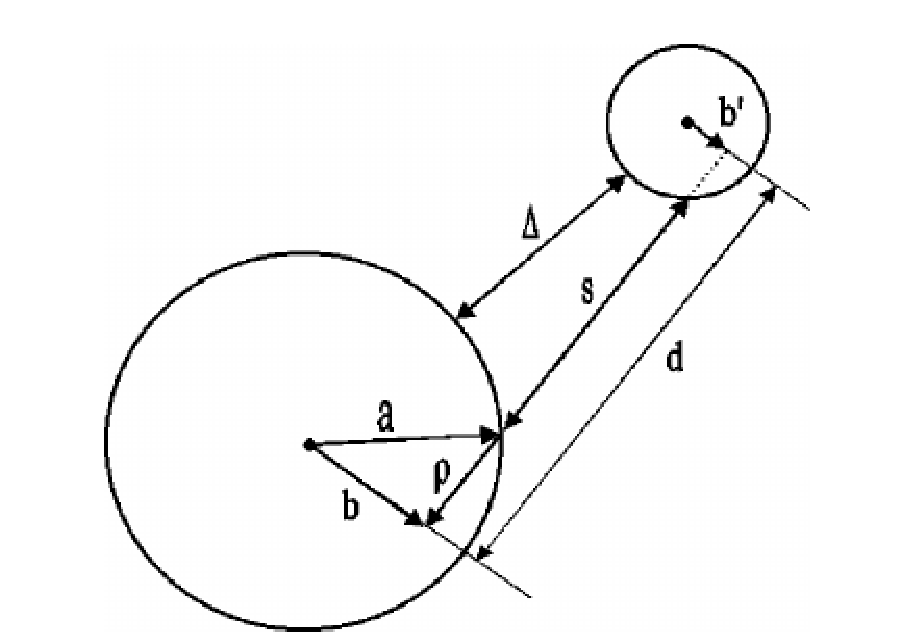
\includegraphics[width=0.45\textwidth]{diffuseKim01_Fig2}
\end{center}
\caption{
	A portion of a path;
}
\label{KimFig2}
\end{figure}

\item[2014-05-12 Predrag to Tingnan]
We need to create our own version of Fig.~4 of \refref{CGS92}.


\item[2014-05-16 Tingnan] I listed my cycles of topological
    length 2 in \reftab{tab:ListLength2}. In \reftab{tab:comparison0}
    and \reftab{tab:comparison1} the results from numerical program are
    compared with exact formula. I will create the new figure.

\begin{table}[htbp]
  \centering
  \caption{Comparison between Tingnan's numerical program and
  the ChaosBook analytic formula
  (\HREF{http://www.streamsound.dk/book1/chaos/chaos.html\#300/z}
  {click here}), for cycle type $\bar{0}$. $\Delta\ExpaEig_e$ and $\Delta t_p$ show the differences of expanding eigenvalue $\ExpaEig$'s and  the period $\period{}$'s}
    \begin{tabular}{|r|r|rr|r|r|}
	\hline
    $\ExpaEig_e$ & $t_p$    & \multicolumn{2}{c|}{disklabel} &\multicolumn{1}{c|}{ $\Delta\ExpaEig_e$} & \multicolumn{1}{c|}{$\Delta t_p$} \\\hline
    4.539722204 & 0.600000 & 0     & 6     &  0     & 0 \\
    4.539722204 & 0.600000 & 2     & 8     &  0     & 0 \\
    4.539722204 & 0.600000 & 4     & 10    &  0     & 0 \\
    33.580485941 & 3.967434 & 1     & 7     &  7.11E-15 & 5.33E-15 \\
    33.580485941 & 3.967434 & 3     & 9     &  7.11E-15 & 5.33E-15 \\
    33.580485941 & 3.967434 & 5     & 11    &  7.11E-15 & 5.33E-15 \\
    \hline
    \end{tabular}%
  \label{tab:comparison0}%
\end{table}%

\begin{table}[htbp]
  \centering
  \caption{Comparison between my numerical program and chaosbook formula  (\HREF{http://www.streamsound.dk/book1/chaos/chaos.html\#300/z}
    {click here}), for cycle type $\bar{1}$. $\Delta\ExpaEig_e$ and $\Delta t_p$ show the differences of expanding eigenvalue $\ExpaEig$'s and  the period $\period{}$'s}
    \begin{tabular}{|r|r|rrr|r|r|}
    \hline
        $\ExpaEig_e$ & $t_p$    & \multicolumn{3}{c|}{disklabel} &\multicolumn{1}{c|}{ $\Delta\ExpaEig_e$} & \multicolumn{1}{c|}{$\Delta t_p$} \\\hline
    26.34522 & 1.703848 & 0     & 4     & 8     & 4.30E-08 & 2.00E-15 \\
    26.34522 & 1.703848 & 2     & 6     & 10    & 5.40E-08 & 2.00E-15 \\
	\hline
    \end{tabular}%
  \label{tab:comparison1}%
\end{table}%


\item[2014-05-18 Predrag to Tingnan] Thanks for checking - your
    numerics is 100\% good, great. I reformatted
    \reftab{tab:ListLength2} - nothing important. For some reason the
    Floquet multipliers for the \cycle{59} set are accurate only to
    $10^{-8}$, even though your check of analytic formulas are good to
    $10^{-15}$. Not a pressing problem at the moment...

\item[2014-05-20 Predrag]
Elementary cell symbolic dynamics labels are not disk labels, but rather
the labels of transitions between disks along the 12 translational
vectors. In \reffig{diskDirectionsElCell} I label the
translation vectors connecting the center of the current disk to the
center of the next disk.

\item[2014-05-21 Tingnan]
I migrated my code base to cpp for
faster computing speed (in order to find periodic orbits of topological
length 8). I will try both derivative-free (Nelder-Mead) routine as well
as those methods based on derivatives. The multi-dimensional flight time
function (to be minimized) seems to have a quite complex landscape which
creates a lot of numerical difficulties. Do you know which references
have figures/tables showing the diffusion coefficient/flight time/etc as
a function of some parameters? Insofar I can only find estimations on
hard disks as a function of disk separation $w$. I am looking at this
because Dan would like to see the parameter variations and their effects,
from an experimental aspect.

\item[2014-05-20 Predrag]
All illustrations seem to be worked out for 1-dimensional maps (see
references toward the beginning of this blog). We would be the first to
compute something for Lorentz billiard, I believe.

\item[2014-05-20 Predrag]
Regarding spherical billiards for Feifei Qian: there is lots of
literature on the web, Google it (though I have not found much). Random
reference: Donnay\rf{Donnay88}
(\HREF{http://chaosbook.org/library/Donnay88.pdf}{click here}).
Programming should be easy; each orbit is a great circle. If the billiard
is a sphere with a reflecting circle drawn on, find the intersection of a
great circle with it, the specularly reflect it around the intersection
point. That seems to say that all orbits (with the exception of the
equator parallel to the billiard wall circle) are marginally stable
period 2. So we need to think of something more interesting, like 2
circular billiard walls, not symmetrically placed...

Totally unrelated:
\HREF{http://www.domerama.com/software/sketchup-3d-models/} {Sketchup}
might be fun to use.


\begin{table}
{\small
%\begin{center}
\begin{tabular}{|r|r|l|l|l|}
\hline
$\period{p}$ & \# cycles & $\zeta$(0,0) & $\lambda$ & D \\ \hline\hline
1      & 0      &   -    &   -  &   - \\
2      & 24     & -0.31697 & 1.330 & 0.750\\
3      & 64     & -0.54152 & 1.435 & 0.677\\
4      & 156    & -0.09718 & 1.902 & 0.565\\
5      & 492    &  0.02383 & 2.324 & 0.425\\
6      & 1484   &  0.02812 & 1.931 & 0.259\\
7      & 5244   &  0.02044 & 1.836 & 0.371\\
8      & 19008  & -0.00036 & 1.754 & 0.513\\ \hline\hline
\multicolumn{3}{|l|}{\refRef{MacZwa83}, estimate}
                           &   -   & 0.175 \\
\multicolumn{3}{|l|}{numerical experiment}
                           & 1.760 & 0.25
\\ \hline
\end{tabular}
\hfill
\begin{tabular}{|r|r|l|l|l|}
\hline
$\period{p}$ & \# cycles & $\zeta$(0,0) & $\lambda$ & D \\ \hline\hline
1      & 0      &   -    &   -  &   - \\
2      & 24     & -0.34807 & 1.312 & 0.379\\
3      & 64     & -0.57736 & 1.418 & 0.343\\
4      & 168    & -0.11233 & 1.909 & 0.285\\
5      & 516    &  0.01399 & 2.408 & 0.202\\
6      & 1589   & -0.01291 & 2.004 & 0.110\\
7      & 5700   & -0.02034 & 1.903 & 0.170\\
8      & 20729  & -0.00109 & 1.785 & 0.240\\
\hline\hline
\multicolumn{3}{|l|}{\HREF{arixv.org/pdf/1202.2904.pdf}{click here}}& - & 0.25 \\
\multicolumn{4}{|l|}{numerical experiment} & 0.25 \\ \hline
\end{tabular}
} %end {\small
\caption{\label{TCELL}
Elementary cell, $w$=0.3.
(left) Schreiber 1992 calculation\rf{CGS92}.
Gaspard 1992 note: ``My numerical estimate for the Lyapunov exponent
when $w=0.3$ is $\lambda = 1.760 \pm 0.002$, which supports the result of
this table.''
(right) Zhang 2014-05-23 calculation, had errors.
For the corrected version, see
\reftab{TCELL2}.
}
%\end{center}
\end{table}

\item[05-23-2014 Tingnan]
I think I in my and Schreiber's numerical calculation for the diffusion
coefficients we have missed the spatial dimension $\nu=2$ at the
denominator \refeq{TS:formula}. Now results are updated in
\reftab{TCELL}. Should we say that now both Lyapunov and diffusion
coefficient are converged?

\item[05-23-2014 Predrag]
Impressive calculation for $\period{}=8$!
You are right about Schreiber missing $\nu=2$; I have it in my overheads.
The number of cycles seems to be creeping
up (from initial Tingnan's \reftab{TCELL1} to the current \reftab{TCELL}.
I doubt I'll ever find the Schreiber's data, it is so long ago...

%My worry is still that the diffusion constant and
%the Lyapunov exponent of \reftab{TCELL1} do not agree for even $\cl{}=2$, so maybe
%I'll have to recompute \refeq{TS:formula} in this case, using your
%\reftab{tab:ListLength2} data.
The convergence for both the Lyapunov and the diffusion
coefficient seem not very good, but let's see well the Lyapunov works out
once you compute it in the fundamental domain.

\item[05-26-2014 Tingnan]
If I am not wrong the zeta function for $n=2$ and $n=3$ cases are just the summation over the weights (using the truncation formula)
\[
\zeta(0,0)=1-\sum_{\cl{p}\leq2,3}t_{p}=1-\sum_{\cl{p}\leq2,3} \frac{1}{\ExpaEig_{p}}
\]
I am starting to compute the cycles in the fundamental domain.
Not sure how to convert the fundamental domain symbols (a-f, A-F) into my program. Are we still trying to use the least action method in the fundamental domain? If so, for each of the symbol, which disks should be included for the computation? In Fig.~5 of Schreiber paper we can see that the number of the disks visited for each symbol
is different. And I am not sure about this sentence in Schreiber's paper:

``The right and left turns are not distinguished - instead,  one reads
off a symbol whether the next turn has to be taken in the same or in the
opposite sense."

\item[2014-05-28 Predrag] Notions `right' and `left' are well defined in
the elementary cell. In the fundamental domain on indicates only the
successive relative orientations: either one turns in the same sense as
in the preceding turn, or one turns in the sense opposite of the
preceding turn. Is that clearer?

\item[2014-05-28 Tingnan] Now it is clearer. Let me see how the fundamental domain cycle could be computed.

\item[05-26-2014 Tingnan]

I spent some effort trying to derive (21.8, 21.9) in ChaosBook  (\HREF{http://www.streamsound.dk/book1/chaos/chaos.html\#445/z}
{click here}), in preparation to compute the dynamical averages in the fundamental domain.

\begin{align*}
\left\langle \phi\vert\Lop(y,x)\vert\rho\right\rangle  &= \int_{M}dy\int_{M}dx\phi(y)\delta(y-f^{t}(x))\rho(x)\\
 &= \sum_{a,b}^{\vert G\vert}\int_{\tilde{M}_{a}}dx\int_{\tilde{M}_{b}}dy\phi(y)\delta(y-f^{t}(x))\rho(x)\\
 &= \sum_{a,b}^{\vert G\vert}\int_{\tilde{M}}d\tilde{x}\int_{\tilde{M}}d\tilde{y}\phi(\mathbf{b}\tilde{y})\delta(\mathbf{b}\tilde{y}-f^{t}(\mathbf{a}\tilde{x}))\rho(\mathbf{a}\tilde{x})\\
 &= \sum_{a,b}^{\vert G\vert}\int_{\tilde{M}}d\tilde{x}\int_{\tilde{M}}d\tilde{y}\phi(\mathbf{b}\tilde{y})\delta(\tilde{y}-\mathbf{b^{-1}}\mathbf{a}f^{t}(\tilde{x}))\rho(\mathbf{a}\tilde{x})\\
 &= \sum_{h,a,b}^{\vert G\vert}\int_{\tilde{M}}d\tilde{x}\int_{\tilde{M}}d\tilde{y}\phi(\mathbf{b}\tilde{y})\delta_{h,b^{-1}a}\delta(\mathbf{h^{-1}}\tilde{y}-f(\tilde{x}))\rho(\mathbf{a}\tilde{x})
\end{align*}
where we have used the fact that $\det \vert a\vert=1$(e.g.
rotation or translation). The product of two group actions $b^{-1}a$
determines the relative ``displacement'' in the group space. We
can then write the evolution operator using the left regular representation
$D(h)_{ba}=\delta h,b^{-1}a$, as:
\[
\Lop(y,x)=\sum_{h,ab}^{\vert G\vert}D(h)_{ba}\delta(\mathbf{h}^{-1}\tilde{y}-f(\tilde{x}))=\sum_{h,ab}^{\vert G\vert}D(h)_{ba}\Lop(\mathbf{h}^{-1}\tilde{y},\tilde{x})
\]
The linear property of the evolution operator could be written as:
\[
\Lop(z,y)\Lop(y,x)=\sum_{hh^{\prime},abb^{\prime}}^{\vert G\vert}D(h^{\prime})_{b^{'}b}D(h)_{ba}\Lop(\mathbf{h}^{\prime-1}\tilde{z},\tilde{y})\Lop(\mathbf{h}^{-1}\tilde{y},\tilde{x})
\]
Note that $D(h^{\prime})_{b^{'}b}D(h)_{ba}$ multiplies as matrices.

The trace formula in the fundamental domain can now been written as:
\begin{align*}
\tr  \Lop &= \int_{\tilde{M}}d\tilde{x}\sum_{h,aa}^{\vert G\vert}D(h)_{aa}\Lop(\mathbf{h}^{-1}\tilde{x},\tilde{x})\\
 &= \int_{\tilde{M}}d\tilde{x}\sum_{h}^{\vert G\vert}\Tr D(h)\Lop(\mathbf{h}^{-1}\tilde{x},\tilde{x})
\end{align*}
\begin{align*}
\tr  \Lop^{2} &= \int_{\tilde{M}}d\tilde{x}\int_{\tilde{M}}d\tilde{y}\sum_{hh^{\prime},ab^{\prime}}^{\vert G\vert}D(h^{\prime})_{ab}D(h)_{ba}\Lop(\mathbf{h}^{\prime-1}\tilde{x},\tilde{y})\Lop(\mathbf{h}^{-1}\tilde{y},\tilde{x})\\
 &= \int_{\tilde{M}}d\tilde{x}\int_{\tilde{M}}d\tilde{y}\sum_{h^{\prime}h}^{\vert G\vert}D(h^{\prime}h)_{aa}\Lop(\mathbf{h}^{\prime-1}\tilde{x},\tilde{y})\Lop(\mathbf{h}^{-1}\tilde{y},\tilde{x})\\
 &= \int_{\tilde{M}}d\tilde{x}\int_{\tilde{M}}d\tilde{y}\sum_{h^{\prime}}^{\vert G\vert}\Tr  D(h^{\prime}h)\Lop(\mathbf{h}^{\prime-1}\tilde{x},\tilde{y})\Lop(\mathbf{h}^{-1}\tilde{y},\tilde{x})\\
 &= \int_{\tilde{M}}d\tilde{x}\sum_{h^{\prime}h\equiv e}^{\vert G\vert}\Tr  D(h^{\prime}h)\Lop(\mathbf{h}^{\prime-1}\tilde{x},\mathbf{h}f(\tilde{x}))\\
 &= \int_{\tilde{M}}d\tilde{x}\sum_{h^{\prime}}^{\vert G\vert}\Tr  D(h^{\prime})\Lop^{2}(\mathbf{h}^{\prime-1}\tilde{x},\tilde{x})
\end{align*}

Next, we will derive the formula for the {\Fd} in the
fundamental domain.
\begin{align*}
\Tr  \Lop^{t} &= \int_{\mathcal{M}}\Lop^{t}(x,x)dx\\
 &= \int_{\tilde{\mathcal{M}}}d\tilde{x}\sum_{h,a}^{G}D_{aa}(h)\delta(\mathbf{h}^{-1}\tilde{x}-f^{t}(\tilde{x}))e^{\beta\cdot A^{t}(\mathbf{a}\tilde{x})}\\
 &= \sum_{h,a}^{G}D_{aa}(h)\int_{\tilde{\mathcal{M}}}d\tilde{x}\delta(\mathbf{h}^{-1}\tilde{x}-f^{t}(\tilde{x}))e^{\beta\cdot A^{t}(\mathbf{a}\tilde{x})}\\
 &= \sum_{a}^{G}D_{aa}(h)\sum_{\tilde{x_{i}}:\mathbf{h}f^{t}(\tilde{x_{i}})=\tilde{x_{i}}}\frac{e^{\beta\cdot A^{t}(\mathbf{a}\tilde{x_{i}})}}{\vert\det (1-\mathbf{h}J^{t}(\tilde{x_{i}}))\vert}\\
 &= \sum_{a}^{G}\sum_{\tilde{x_{i}}:f^{t}(\tilde{x_{i}})=\tilde{x_{i}}}\frac{e^{\beta\cdot A^{t}(\mathbf{a}\tilde{x_{i}})}}{\vert\det (1-J^{t}(\tilde{x_{i}}))\vert}
\end{align*}
Now I seem to run into an issue: the trace only depends on those
standing global orbits, and it does not take any contributions from
those runaway orbits.

\item[2014-05-28 Predrag]
That's why I spent two weeks fumbling to derive trace formulas in
presence of symmetries: `running orbits' are the \rpo s associated with
the translations of the hexagonal lattice. Ask Xiong Ding to explain
this. He understands the discrete case, is still trying to understand the
continuous symmetry case. In other words, why does Kronecker delta take
values 0 or 1, but the Dirac delta function has values 0 or $\infty$ :)

\item[2014-05-28 Tingnan]

I got it!

A careful re-derivation of the trace formula gives
\begin{align*}
\mathrm{Tr}\mathcal{L} & =\int dx\int dy\delta(x-y)\mathcal{L}(y,x)\\
 & =\vert G\vert^{2}\int_{\tilde{\mathcal{M}}}d\tilde{x}\int_{\tilde{\mathcal{M}}}d\tilde{y}\frac{1}{\vert G\vert}\sum_{a}\frac{1}{\vert G\vert}\sum_{b}\delta(\mathbf{a}\tilde{x}-\mathbf{b}\tilde{y})\mathcal{L}(\mathbf{b}\tilde{y},\mathbf{a}\tilde{x})\\
 & =\vert G\vert^{2}\int_{\tilde{\mathcal{M}}}d\tilde{x}\int_{\tilde{\mathcal{M}}}d\tilde{y}\frac{1}{\vert G\vert}\sum_{a}\frac{1}{\vert G\vert}\sum_{b}\delta(\mathbf{a}\tilde{x}-\mathbf{b}\tilde{y})\delta(\tilde{y}-\mathbf{b^{-1}a}f^{t}(\tilde{x}))\\
 & =\vert G\vert^{2}\int_{\tilde{\mathcal{M}}}d\tilde{x}\int_{\tilde{\mathcal{M}}}d\tilde{y}\underbrace{\frac{1}{\vert G\vert}\sum_{a}}\frac{1}{\vert G\vert}\sum_{h}\delta(\tilde{y}-\mathbf{h}\tilde{x})\delta(\tilde{y}-\mathbf{h}f^{t}(\tilde{x}))\\
 & =\vert G\vert^{2}\int_{\tilde{\mathcal{M}}}d\tilde{x}\int_{\tilde{\mathcal{M}}}d\tilde{y}\frac{1}{\vert G\vert}\sum_{h}\delta(\tilde{y}-\mathbf{h}\tilde{x})\delta(\tilde{y}-\mathbf{h}f^{t}(\tilde{x}))\\
 & =\vert G\vert\int_{\tilde{\mathcal{M}}}d\tilde{x}\sum_{h}\delta(\tilde{x}-\mathbf{h}f^{t}(\tilde{x}))
\end{align*}

The trick is within the double delta function that I previously ignored: both of them would contribute when integrating over $\tilde{y}$.

For the modified evolution operator the trace in the fundamental domain, we now have:

\begin{align*}
\mathrm{Tr}\mathcal{L}^{t} & =\vert G\vert^{2}\int_{\tilde{\mathcal{M}}}d\tilde{x}\int_{\tilde{\mathcal{M}}}d\tilde{y}\frac{1}{\vert G\vert}\sum_{a}\frac{1}{\vert G\vert}\sum_{b}\delta(\mathbf{a}\tilde{x}-\mathbf{b}\tilde{y})\mathcal{L}(\mathbf{b}\tilde{y},\mathbf{a}\tilde{x})\\
 & =\vert G\vert^{2}\int_{\tilde{\mathcal{M}}}d\tilde{x}\int_{\tilde{\mathcal{M}}}d\tilde{y}\frac{1}{\vert G\vert}\sum_{a}\frac{1}{\vert G\vert}\sum_{b}\delta(\mathbf{b^{-1}a}\tilde{x}-\tilde{y})\delta(\tilde{y}-\mathbf{b^{-1}a}f^{t}(\tilde{x}))e^{\beta\cdot A^{t}(\mathbf{a}\tilde{x})}\\
 & =\vert G\vert\int_{\tilde{\mathcal{M}}}d\tilde{x}\int_{\tilde{\mathcal{M}}}d\tilde{y}\sum_{h}\delta(\tilde{y}-\mathbf{h}\tilde{x})\delta(\tilde{y}-\mathbf{h}f^{t}(\tilde{x}))\frac{1}{\vert G\vert}\sum_{a}e^{\beta\cdot A^{t}(\mathbf{a}\tilde{x})}\\
 & =\vert G\vert\int_{\tilde{\mathcal{M}}}d\tilde{x}\sum_{h}\delta(\tilde{x}-\mathbf{h}f^{t}(\tilde{x}))\frac{1}{\vert G\vert}\sum_{a}e^{\beta\cdot A^{t}(\mathbf{a}\tilde{x})}
\end{align*}

I see the trouble more clearly as indicated in the previous blogs: The
averaging over the space group (a point group action followed by a
translation). I think in Pavel's approach we still needs to worry
because his three group actions do not commute with each other?

\item[05-26-2014 Tingnan to Pavel]

Here I put some essential ideas of dynamical averaging. This section could be though as a short version of what has been covered from Chapter 17 to 20 in the book.

Put the quantity that needs to be averaged to exponential
\[
\left\langle e^{\beta\cdot A^{t}}\right\rangle =\frac{1}{\vert M\vert}\int dxe^{\beta\cdot A^{t}(x)}
\]
where $A^{t}(x)=\int_{0}^{t}d\tau a[f^{t}(x)]$. When divided by $t$
this gives the time average. The quantity we are interested can be
obtained by partial differentiation:
\[
\left\langle A^{t}\right\rangle =\frac{\partial}{\partial\beta}\left.\left\langle e^{\beta\cdot A^{t}}\right\rangle \right|_{\beta=0}
\]
The term $\left\langle e^{\beta\cdot A^{t}}\right\rangle $ is expected
to grow exponentially in time and is dominated by the leading eigenvalue
of the evolution operator:
\[
\left\langle e^{\beta\cdot A^{t}}\right\rangle \to(\mathrm{const})e^{ts(\beta)}
\]
The function $s(\beta)=\lim_{t\to\infty}\frac{1}{t}\ln\left\langle e^{\beta\cdot A^{t}}\right\rangle $
is related to the observable as:
\begin{align*}
\left.\frac{\partial s}{\partial\beta}\right|_{\beta=0} & =\lim_{t\to\infty}\frac{1}{t}\left.
\frac{\partial\ln\left\langle e^{\beta\cdot A^{t}}\right\rangle }
     {\partial\beta}\right|_{\beta=0}
   =\lim_{t\to\infty}\frac{1}{t}\left\langle A^{t}\right\rangle \\
 & =\left\langle a\right\rangle
\end{align*}
In order to evaluate $s(\beta)$ we will examine the modified  evolution
operator:
\[
\Lop^{t}(y,x)=\delta(y-f^{t}(x))e^{\beta\cdot A^{t}(x)}
\]
It is a linear operator and has its eigen ``vectors'' (in the function
space) and corresponding eigenvalues:
\[
[\Lop^{t}\rho_{\beta}](y)=\int_{\mathcal{M}}dx\delta(y-f^{t}(x))e^{\beta\cdot A^{t}(x)}\rho_{\beta}(x)=e^{ts(\beta)}\rho_{\beta}(y)
\]

So now we turn the problem into: how can be determine the eigenvalues
(the leading one) in the infinite functional space? We can do that
with the help of spectral determinant. Suppose we have discrete mappings
and set $\Lop\equiv\Lop^{1}$. By evaluating the zeros
of the determinant
\[
\det (1-z\Lop)=\prod_{k}(1-z \lambda_{k})
\]
one can get all eigenvalues $\lambda_{k}$s of the linear operator.
The LHS can be rewritten as exponentials:
\[
\det (1-z\Lop)=\exp\left(-\sum_{n}^{\infty}\frac{z^{n}}{n}\Tr  \Lop^{n}\right)
\]
Now the cycle expansion will help us determine the trace of the linear
operator.

\begin{align*}
\Tr  \Lop^{n} & =\int_{\mathcal{M}}\Lop^{n}(x,x)dx=\int_{\mathcal{M}}dx\delta(x-f^{n}(x))e^{\beta\cdot A^{n}(x)}\\
 & =\sum_{x_{i}:f^{n}(x_{i})=x_{i}}\frac{e^{\beta\cdot A^{n}(x_{i})}}{\vert\det (1-J^{n}(x_{i}))\vert}
\end{align*}
The summation is over all the periodic orbits of length $n$. We may
write it in terms of prime (distinct) periodic orbits:
\[
\Tr  \Lop^{n}=\sum_{p}\cl{p}\sum_{r=1}^{\infty}
\frac{e^{\beta\cdot rA_{p}}}{\vert\det (1-J_{p}^{r})\vert}\delta n,\cl{p}r
\]
where $r$ is the repeat, and $\cl{p}$ is the length of the
prime orbit. A fact: prime periodic orbit of length $\cl{p}$ will
contribute to the sum $\cl{p}$ times for each of the points along
the orbit. Now substitute the trace formula to the determinant, the
summation over $n$ removes the awkward delta function:
\begin{align*}
\det (1-z\Lop) & =\exp\left(-\sum_{n}^{\infty}\frac{z^{n}}{n}\Tr  \Lop^{n}\right)\\
 & =\exp\left(-\sum_{n}^{\infty}\frac{z^{n}}{n}\sum_{p}\cl{p}\sum_{r=1}^{\infty}\frac{e^{\beta\cdot rA_{p}}}{\vert\det (1-J_{p}^{r})\vert}\delta n,\cl{p}r\right)\\
 & =\exp\left(-\sum_{p}\sum_{r=1}^{\infty}\frac{1}{r}\frac{z^{\cl{p}r}e^{\beta\cdot rA_{p}}}{\vert\det (1-J_{p}^{r})\vert}\right)
\end{align*}
So far the {\Fd} is exact. If we are interested only in its leading
zero, it can be approximated by keeping only the expanding
eigenvalues of the {\jacobianM},
\begin{align*}
\vert\det (1-J_{p}^{r})\vert
 & =\left|\prod_{e}(1-\ExpaEig_{p,e}^{r})\prod_{c}(1-\ExpaEig_{p,c}^{r})\right|
 =\vert\ExpaEig_{p}\vert^{r}\left|\prod_{e}(1-\frac{1}{\ExpaEig_{p,e}^{r}})
                                  \prod_{c}(1-\ExpaEig_{p,c}^{r})\right|\\
 & =\vert\ExpaEig_{p}\vert^{r}
\,,
\end{align*}
where $\ExpaEig_{p}$ is the product of all the expanding
eigenvalues. In this way the {\Fd} is approximated by the {\dzeta}:
\begin{align*}
\frac{1}{\zeta(z,\beta)} & =\exp\left(-\sum_{p}\sum_{r=1}^{\infty}\frac{1}{r}\frac{z^{\cl{p}r}e^{r\beta\cdot A_{p}}}{\vert\ExpaEig_{p}\vert^{r}}\right)\\
 & =\exp\left(-\sum_{p}\sum_{r=1}^{\infty}\frac{1}{r}t_{p}^{r}\right)
   =\exp\left(\sum_{p}\ln(1-t_{p})\right)\\
 & =\prod_{p}(1-t_{p})
\,,
\end{align*}
where
\[
t_{p}=\frac{z^{\cl{p}}e^{\beta\cdot A_{p}}}{\vert\ExpaEig_{p}\vert}
\,.
\]
is the weight associated with each prime cycle (for flows we
replace $z$ with $e^{-s}$ and $\cl{p}$ with $\period{p}$). For each
$\beta$, the zeros of {\dzeta}s could be evaluated
numerically.

\item[2014-05-28 Tingnan]
\begin{table}
{\small
%\begin{center}
\begin{tabular}{|r|r|l|l|l|}
\hline
$\period{p}$ & \# cycles & $\zeta$(0,0) & $\lambda$ & D \\ \hline\hline
1      & 0      &   -    &   -  &   - \\
2      & 24     & -0.31697 & 1.330 & 0.750\\
3      & 64     & -0.54152 & 1.435 & 0.677\\
4      & 156    & -0.09718 & 1.902 & 0.565\\
5      & 492    &  0.02383 & 2.324 & 0.425\\
6      & 1484   &  0.02812 & 1.931 & 0.259\\
7      & 5244   &  0.02044 & 1.836 & 0.371\\
8      & 19008  & -0.00036 & 1.754 & 0.513\\ \hline\hline
\multicolumn{3}{|l|}{\refRef{MacZwa83}, estimate}
                           &   -   & 0.175 \\
\multicolumn{3}{|l|}{numerical experiment}
                           & 1.760 & 0.25
\\ \hline
\end{tabular}
\hfill
\begin{tabular}{|r|r|l|l|l|}
\hline
$\period{p}$ & \# cycles & $\zeta$(0,0) & $\lambda$ & D \\ \hline\hline
1      & 0      &   -    &   -  &   - \\
2      & 24     & -0.31697 & 1.330 & 0.375\\
3      & 64     & -0.54152 & 1.435 & 0.339\\
4      & 168    & -0.09764 & 1.902 & 0.284\\
5      & 516    &  0.02334 & 2.324 & 0.215\\
6      & 1589   & -0.00481 & 1.975 & 0.133\\
7      & 5700   & -0.01241 & 1.885 & 0.184\\
8      & 20729  & -0.01006 & 1.785 & 0.247\\
\hline\hline
\multicolumn{3}{|l|}{\HREF{arixv.org/pdf/1202.2904.pdf}{click here}}& - & 0.25 \\
\multicolumn{4}{|l|}{numerical experiment} & 0.25 \\ \hline
\end{tabular}
} %end {\small
\caption{\label{TCELL2}
Elementary cell, $w$=0.3.
(left) Schreiber 1992 calculation\rf{CGS92}.
Gaspard 1992 note: ``My numerical estimate for the Lyapunov exponent
when $w=0.3$ is $\lambda = 1.760 \pm 0.002$, which supports the result of
this table.''
(right) Zhang 2014-05-28 calculation.
}
\end{table}

From the table \reftab{TCELL2} we can see that convergence does not
improve. I also included the elementary cell 2-cycles
\reftab{tab:length2withfloquet}, with updated numerical values as well as
the Floquet multipliers.

I also tried to compute the diffusion coefficients for other parameters
(e.g., $w=0.2$). Then I noticed that I can get negative values for
Lyapunov exponents (as sometimes $T$ averaged from the truncation could
be negative). Is it something normal (because of pruning)?

\item[2014-05-28 Predrag]
I believe that for cycle expansions that are too truncated negative
Lyapunovs are possible, because all  fundamental cycles have not been
accounted for yet.

The diffusion constant computed from cycles of length 6 is still
worrisome. We need to understand what happens here. Has the average time
in the numerator of the {\cycForm} \refeq{TS:formula} suddenly jumped
because of the new length 6 periodic orbit, of multiplicity 2?
(See \refFig{7diskFundDflips2A}\,(c).)
This cycle is a fixed point in the fundamental domain, so taken care of
in the very first level of computation; there is nothing funny going on
at length 6 in \reftab{TS:CONV}.

%%%%%%%%%%%%%%%%%%%%%%%%%%%%%%%%%%%%
\input tabListLength2
%%%%%%%%%%%%%%%%%%%%%%%%%%%%%%%%%%%%

%%%%%%%%%%%%%%\item[Figure ?]%%%%%%%%%%%%%%%%%%%%%%%%%%%%%%%%%%%%%%%%%%
\begin{figure}
\begin{center}
(a)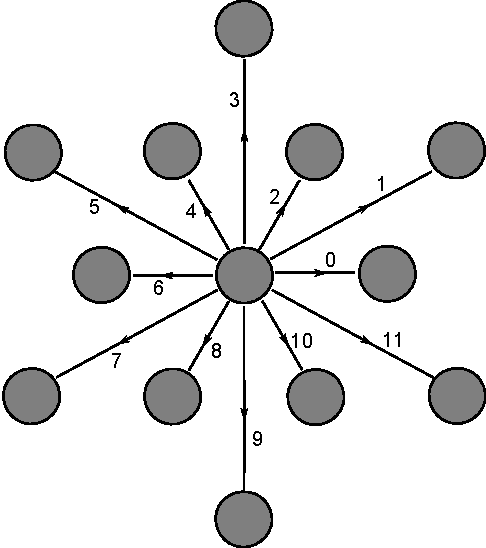
\includegraphics[width=0.29\textwidth]{diffuseDiskDirectionsElCell}
(b)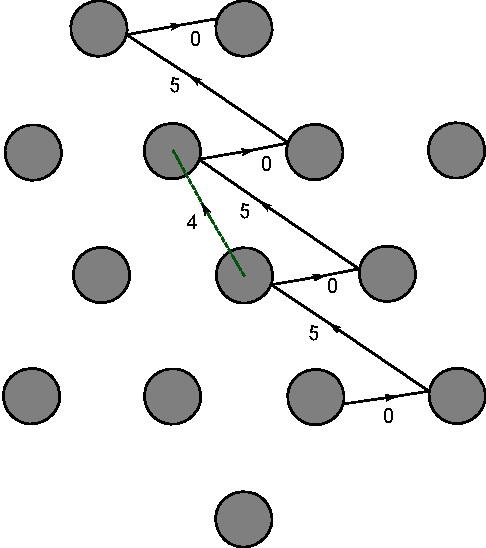
\includegraphics[width=0.29\textwidth]{diffuseDiskDirecsElCell05}
(c)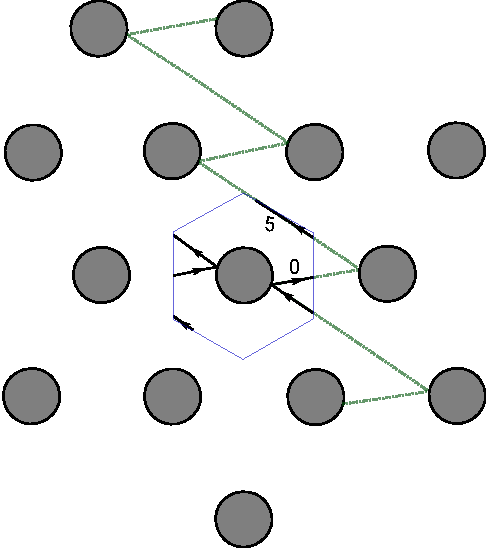
\includegraphics[width=0.29\textwidth]{diffuseDiskDirecsElCell05red}
\end{center}
\caption{
Elementary cell symbolic dynamics is obtained by labeling the translation
vectors connecting the center of the current disk to the center of the
next disk.
(a) The finite horizon is here imposed by limiting jumps from the
center cell to only the short jumps (six even labels $0, 2,\cdots,10$)
and the `long jumps' (six odd labels $1, 3,\cdots,11$).
(b) Running mode \cycle{05} advances by $\hn_4$ per period.
(c) In the elementary cell this is a \po\ \cycle{05}
    of topological length 2.
    }
\label{diskDirectionsElCell}
\end{figure}
%%%%%%%%%%%%%%\item[Figure 4]%%%%%%%%%%%%%%%%%%%%%%%%%%%%%%%%%%%%%%%%%%

\item[05-30-2014 Tingnan]
I listed in \reftab{tab:addlabel} all the intermediate quantities. The
sudden jump of diffusion coefficient is from the decrease of the mean
lattice displacement.

\begin{table}[htbp]
  \centering
  \caption{\Dzeta\ cycle expansion estimates of
  the mean flight time
  $\spaceAver{\period{}}_\zeta
  =\sum^{\prime}(-1)^{k}(\tau_{p_1}+\cdots+\tau_{p_k})/\vert\ExpaEig_{p_1}\cdots\ExpaEig_{p_k}\vert$,
  mean log of the expanding Floquet multiplier
  $\spaceAver{\ln\ExpaEig}_\zeta
  =\sum^{\prime}(-1)^{k}(\mu_{p_1}+\cdots+\mu_{p_k})/\vert\ExpaEig_{p_1}\cdots\ExpaEig_{p_k}\vert$,
  and thee diagonal components of the diffusion tensor,
  $\spaceAver{n_{x}n_{x}}
    =\sum^{\prime}(-1)^{k}(n_{xp_1}^2+\cdots+n_{xp_k}^2)/\vert\ExpaEig_{p_1}\cdots\ExpaEig_{p_k}\vert$}.
    \begin{tabular}{c|r|r|r|r}
    $n_p$ & $\spaceAver{\period{}}_\zeta$
               & $\spaceAver{\ln\ExpaEig}_\zeta$
                        & $\spaceAver{n_{x}n_{x}}$
                                 & $\spaceAver{n_{y}n_{y}}$ \\
    \hline
    2 & 2.3971 & 3.1891 & 1.7998 & 1.7998 \\
    3 & 2.8949 & 4.1552 & 1.9615 & 1.9615 \\
    4 & 1.0728 & 2.0409 & 0.6086 & 0.6086 \\
    5 & 0.5249 & 1.2198 & 0.2260 & 0.2260 \\
    6 & 0.6523 & 1.2884 & 0.1721 & 0.1750 \\
    7 & 0.7112 & 1.3408 & 0.2595 & 0.2625 \\
    8 & 0.7011 & 1.2513 & 0.3461 & 0.3455 \\
    \end{tabular}%
  \label{tab:addlabel}%
\end{table}

\item[2014-05-31 Predrag]
If you ever need to argue that one must reduce the symmetry,
\reftab{tab:addlabel} is your argument. In the elementary cell at
$\cl{}=6$ you pick up \cycle{0\underline{10}8642} and
\cycle{02468\underline{10}}. Try removing them from the sum for
$\spaceAver{\cl{}}_\zeta$: does the mean flight time jump? In the
fundamental domain this short period cycle is a fixed point, accounted
for in the very first step of the calculation.

At $\cl{}=4$  the mean flight time drops precipitously because of
short period cycles such as
\cycle{\underline{10}842}
(see \reffig{schreiberFig3})?

At $\cl{}=5$  the mean flight time is halved again, because of
what short cycles? Can you check if there are 5-cycles with 5 even symbols?

For jumps in the diffusion coefficient the decrease of the mean
lattice displacement presumably comes from running orbits composed
only of short hops - I cannot visualize those, you should check what they look
like in your data set.

Somewhere in Landau \&\ Lifshitz there is a theorem that says (directly
or indirectly) that the diffusion tensor on the hexagonal lattice is
isotropic. (That is not the case on a square lattice - diagonals
$\spaceAver{n_{x}n_{y}}$ are different from $\spaceAver{n_{x}n_{x}}$).
One can probably find the proof or a reference to the theorem in the
literature on lattice gases in 2 dimensions. If that is true, Tingnan's
$\cl{}=6$, $\cl{}=7$ and $\cl{}=8$ are still to be debugged.


\item[2014-06-02 Tingnan]
Let us expand the $\spaceAver{\period{}}_\zeta$ explicitly to a few
orders, e.g., 4th and 5th order:
\begin{align*}
\spaceAver{\period{}}_\zeta
  &=\sum^{\prime}(-1)^{k}(\tau_{p_1}+\cdots+\tau_{p_k})/\vert\ExpaEig_{p_1}\cdots\ExpaEig_{p_k}\vert\\
  &=(-1)\left(\sum^{n_p\leq5}\frac{\tau_{p_k}}{\vert\ExpaEig_{p_k}\vert} - \sum^{n_{p_{k1}}+n_{p_{k2}}\leq5}\frac{\tau_{p_{k1}}+\tau_{p_{k2}}}{\vert\ExpaEig_{p_{k1}}\ExpaEig_{p_{k2}}\vert} \right)\\
  &=(-1)\left(\underbrace{2.397115663}_{n_p=2} + \underbrace{0.497760092}_{n_p=3} + \underbrace{1.176239465}_{n_p=4} + \underbrace{0.645962664}_{n_p=5}\right.\\
  &\phantom{{}=(-1)}\left.\underbrace{-2.998326076}_{n_{p_1}=2,n_{p_2}=2} - \underbrace{1.193809754}_{n_{p_1}=2,n_{p_2}=3}\right)
\,,
\end{align*}

From what I see, beginning from $n=4$ the pseudo-cycles (in our case
composed of two short prime cycles) start to contribute to the space
averages, and their contributions are larger than those of prime cycles
of the same topological length. Many cycles have long topological length
but short flight time, I will try to identify a few of those.

Beginning from $n=6$, I am missing cycles that are very close to the
tangent, because sometimes the path intersects with a disk due to slight
numerical differences. Say if a cycle is of multiplier $12$ due to
rotational symmetry, I sometimes only find 11 or 10 from this family.
Again, this is probably another argument of why we needs to go to the
fundamental domain.

\item[2014-07-14 Tingnan]
I think we should propose a separate label $\circ$ to indicate the
collision on the disk, i.e. $\cycle{\circ f}=\cycle{06}$. Without the
additional symbol, when we are doing the string reduction things could go
wrong.

The topological robustness of the cycle inspired me to look at the cycle
in fundamental domain from a different perspective. Before we write the
explicit symbol string using the 3 generators, let us just visualize a
flight between two nearest disk. I label the triangular pieces with
numbers, \reffig{fig:topoCombo}. A flight between two disk can be
represented by the combination of two labels (numbers). With symmetry
been considered, there are 12 topologically distinct combinations (out of
18 possible combinations):
\bea
1-1 & 1-1^\prime\continue
1-2 & 1-2^\prime\continue
1-3 & 1-3^\prime\continue
2-2 & 2-2^\prime\continue
2-3 & 2-3^\prime\continue
3-3 & 3-3^\prime
\eea
\begin{figure}
\begin{center}
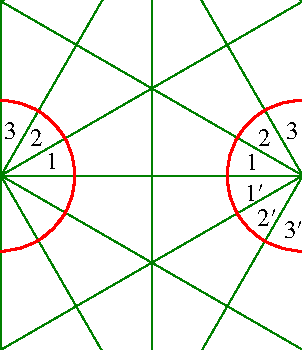
\includegraphics[width=0.5\textwidth]{diffuseTopologicalCombinationZoom}
\end{center}
\caption{Topological combination of fundamental domains.}
\label{fig:topoCombo}
\end{figure}
Now a fundamental domain fixed point should correspond to a symmetric (or
anti-symmetric) combination:
\bea
\cycle{f\circ} &= 1-1 &= \cycle{06}\continue
\cycle{sf\circ} &= 2-2^\prime &= \cycle{08}\continue
\cycle{\ell f\circ} &= 2-2 &= \cycle{048} \continue
\cycle{s\ell fs\ell\circ} &= 3-3^\prime &= \cycle{02}\continue
\cycle{s\ell f\ell\circ} &= 3-3 &= \cycle{0\underline{10}8642}\continue
\eea
The unknown fixed point then corresponds to $1-1^\prime$ which actually
degenerates with $1-1$. Though those orbits would fall at the boundary of
the fundamental domain, I choose the label such that the orbit minimize
the flight time between the labeled triangular pieces. Similarly we can
generate 12 possibilities for long flights.

\item[2014-09-17 Tingnan]

% Preview source code from paragraph 0 to 6

Following the previous section, for a prime periodic orbit $\tilde{p}=\tilde{x}_{0}\cdots\tilde{x}_{n_{p}-1}$(of
length $n_{p}$), in the fundamental domain $\tilde{\Omega}=[0,\pi/6]\times[-pi/2,pi/2]$,
the total displacement in the full space $\hat{\Omega}$ after traveling
along the cycle one time is given by:
\[
\hat{n}_{\tilde{p}}(\tilde{x}_{0})=\sum_{j=0}^{\vert\tilde{p}\vert-1}\hat{n}(\tilde{x}_{j},g_{\tilde{p}}(\tilde{x}_{j},\tilde{x}_{0}))=\sum_{j=0}^{\vert\tilde{p}\vert-1}g_{\tilde{p}}(\tilde{x}_{j},\tilde{x}_{0})\circ\hat{n}(\tilde{x}_{j},e),
\]
where $g_{\tilde{p}}(\tilde{x}_{j},\tilde{x}_{0})$ is cumulated point
group operations when travels to $\tilde{x}_{j}$ if we start from
$\tilde{x}_{0}$ and $\hat{n}(\tilde{x},e)$ gives the diplacement
of one free flight if start from$x=(\tilde{x},e)$. We have a recursive
relation:
\[
g_{\tilde{p}}(\tilde{x}_{j},\tilde{x}_{0})=\begin{cases}
1 & {\rm \quad if\quad}j=0\\
\gamma(\tilde{x}_{j-1},g_{\tilde{p}}(\tilde{x}_{j-1},\tilde{x}_{0})) & {\rm \quad if\quad}j\geq1
\end{cases},
\]
where the function $\gamma(\tilde{x},g)=g\circ\gamma(\tilde{x},e)$,
gives the point group operations after one free flight $f(x)$ for
any points $x=(\tilde{x},g)$ in the elementary cell $\Omega$. Let
$g_{j}\equiv\gamma(\tilde{x_{j}},e)$, then
\begin{align*}
g_{\tilde{p}}(\tilde{x}_{j},\tilde{x}_{0}) & =g_{\tilde{p}}(\tilde{x}_{j-1},\tilde{x}_{0})\circ\gamma(\tilde{x}_{j-1},e)\\
 & =g_{\tilde{p}}(\tilde{x}_{j-2},\tilde{x}_{0})\circ\gamma(\tilde{x}_{j-2},e)\circ\gamma(\tilde{x}_{j-1},e)\\
 & =1\circ g_{0}\circ\cdots\circ g_{j-1}
\end{align*}
We notice that the displacement depends on the starting point of the
cycle. The total group action after we return to $\tilde{x}_{0}$
along the cycle is $g_{\tilde{p}}(\tilde{x}_{0})=g_{0}\circ g_{1}\cdots\circ g_{n_{p}-1}$.
If we start from another point on the cycle, for example $\tilde{x}_{1}$,
then the total group action after we went through the cycle is $g_{\tilde{p}}(\tilde{x}_{1})=g_{1}\circ g_{2}\cdots\circ g_{n_{p}-1}\circ g_{0}=g_{0}^{-1}\circ g_{\tilde{p}}(\tilde{x}_{0})\circ g_{0}$,
i.e. they are in the same conjugacy class of the point group $C_{6v}$,
and thus they have the same order number. This intuitively makes sense:
the number of repeats takes for the fundamental domain cycle to form
an elementary cell cycle, should be independent of its starting point.

We can also derive the relation between the net displacement traveled
along the cycle, if we start from different point (say, $\tilde{x}_{1}$):
\[
\hat{n}_{\tilde{p}}(\tilde{x}_{1})=g_{0}^{-1}\circ\left(\hat{n}_{\tilde{p}}(\tilde{x}_{0})+g_{\tilde{p}}(\tilde{x}_{0})\circ\hat{n}(\tilde{x}_{0},e)-\hat{n}(\tilde{x}_{0},e)\right).
\]
This relationship is nontrivial. Please note that $\vert\hat{n}_{\tilde{p}}(\tilde{x}_{0})\vert\neq\vert\hat{n}_{\tilde{p}}(\tilde{x}_{0})\vert$
in general. But suppose $g_{\tilde{p}}(\tilde{x}_{0})$ belongs to
a relflection class ($\sigma_{v}$ or $\sigma_{d}$) so that $g_{\tilde{p}}(\tilde{x}_{0})\circ g_{\tilde{p}}(\tilde{x}_{0})=e$,
the displacement of the elementary cell cycle is:
\begin{align*}
\hat{n}_{\tilde{p}}(\tilde{x}_{1})+g_{\tilde{p}}(\tilde{x}_{1})\circ\hat{n}_{\tilde{p}}(\tilde{x}_{1})= & g_{0}^{-1}\circ\left(\hat{n}_{\tilde{p}}(\tilde{x}_{0})+g_{\tilde{p}}(\tilde{x}_{0})\circ\hat{n}(\tilde{x}_{0},e)-\hat{n}(\tilde{x}_{0},e)\right)\\
 & +g_{0}^{-1}\circ g_{\tilde{p}}(\tilde{x}_{0})\circ\left(\hat{n}_{\tilde{p}}(\tilde{x}_{0})+g_{\tilde{p}}(\tilde{x}_{0})\circ\hat{n}(\tilde{x}_{0},e)-\hat{n}(\tilde{x}_{0},e)\right)\\
= & g_{0}^{-1}\circ(\hat{n}_{\tilde{p}}(\tilde{x}_{0})+g_{\tilde{p}}(\tilde{x}_{0})\circ\hat{n}(\tilde{x}_{0},e)-\hat{n}(\tilde{x}_{0},e)\\
 & +g_{\tilde{p}}(\tilde{x}_{0})\circ\hat{n}_{\tilde{p}}(\tilde{x}_{0})+\hat{n}(\tilde{x}_{0},e)-g_{\tilde{p}}(\tilde{x}_{0})\circ\hat{n}(\tilde{x}_{0},e))\\
= & g_{0}^{-1}\circ\left(\hat{n}_{\tilde{p}}(\tilde{x}_{0})+g_{\tilde{p}}(\tilde{x}_{0})\circ\hat{n}_{\tilde{p}}(\tilde{x}_{0})\right)
\end{align*}


If $g_{\tilde{p}}(\tilde{x}_{0})$ belongs to a rotation class, the
corresponding elementary cell cycle has a net displacement of zero
(i.e. the orbit is stationary); so only those orbits that belongs
to $(e,\sigma_{v},\sigma_{d})$ are running orbits in the full space.
We can define the quantity:
\[
\hat{N}_{\tilde{p}}(\tilde{x}_{0})=\lim_{m\to\infty}\frac{1}{m}\sum_{j=0}^{m-1}g_{\tilde{p}}^{j}(\tilde{x}_{0})\hat{n}_{\tilde{p}}(\tilde{x}_{0})
\]


The limit exists, and can be understood as the effective displacement
of the fundamental domain cycle, when started from the point$\tilde{x}_{0}$.
For rotationa type of fundamental domain cycle it is always $0$;
for reflection type of cycle it is the displacement projected to the
symmetry line direction (which should also be the travel direction
of the corresponding elementary domain cycle). We would like to use
this in the zeta function because, if we travel along a fundamental
domain cycle $r$ times, the result is just $r\hat{N}_{\tilde{p}}(\tilde{x}_{0})$.

The unweighed $\zeta$ function can be written as:
\[
{\rm Tr}\mathcal{L}^{n}=\sum_{\tilde{p}}\delta n,n_{\tilde{p}}r\frac{\sum_{j=0}^{n_{\tilde{p}}-1}e^{r\beta\cdot w(\tilde{x}_{j})\circ\hat{N}_{\tilde{p}}(\tilde{x}_{j})}}{\vert\Lambda_{\tilde{p}}\vert^{r}}
\]
where the weight $w(\tilde{x}_{j})\in G$ the point group. I would
argue that because the number points on a fundamental domain cycle
could be any integer, the sum
\[
\sum_{j=0}^{n_{\tilde{p}}-1}w(\tilde{x}_{j})\circ\hat{N}_{\tilde{p}}(\tilde{x}_{j})
\]


could be made to zero with many different choice of weights.

If I choose $w(\tilde{x}_{j})$ such that $w(\tilde{x}_{j})\circ\hat{N}_{\tilde{p}}(\tilde{x}_{j})\equiv\hat{N}_{\tilde{p}}(\tilde{x}_{0})\equiv\hat{N}_{\tilde{p}0}$
for now, and we will try to figure out how to add the group characters
to the zeta function. Now with the choice of weight, the trace is
written as:
\[
{\rm Tr}\mathcal{L}^{n}=\sum_{\tilde{p}}n_{\tilde{p}}\sum_{r=1}^{\infty}\delta n,n_{\tilde{p}}r\frac{e^{r\beta\cdot\hat{N}_{\tilde{p}0}}}{\vert\Lambda_{\tilde{p}}\vert^{r}}
\]
which is simple but does not give a zero average displacement.


\item[2014-10-01 Tingnan]
% Preview source code from paragraph 0 to 4

Starting from the group projection operator:
\[
P_{\alpha}=\frac{d_{\alpha}}{\vert G\vert}\sum_{h\in G}\chi_{\alpha}(h)\mathbf{h}^{-1}
\]


We may write the trace formula as :
\[
\mathrm{tr}\mathcal{L}^{n}=\sum_{\alpha}\mathrm{tr}\mathcal{L}_{\alpha}^{n}
\]
With
\begin{align*}
\mathrm{tr}\mathcal{L}_{\alpha}^{n} & =P_{\alpha}\int_{\mathcal{M}}dx\mathcal{L}^{n}(x,x)\\
 & =P_{\alpha}\sum_{a\in G}\int_{\mathcal{\tilde{\mathcal{M}}}}d(a\tilde{x})\mathcal{L}^{n}(a\tilde{x},a\tilde{x})\\
 & =P_{\alpha}\sum_{a\in G}\int_{\mathcal{\tilde{\mathcal{M}}}}d\tilde{x}\mathcal{L}^{n}(a\tilde{x},a\tilde{x})\\
 & =P_{\alpha}\sum_{a\in G}\int_{\mathcal{\tilde{\mathcal{M}}}}d\tilde{x}\delta(a\tilde{x}-f^{n}(a\tilde{x}))e^{\beta\cdot\hat{n}_{(n)}(a\tilde{x})-sT_{(n)}(a\tilde{x})}\\
 & =P_{\alpha}\sum_{a\in G}\int_{\mathcal{\tilde{\mathcal{M}}}}d\tilde{x}\delta(\tilde{x}-f^{n}(\tilde{x}))e^{\beta\cdot a\cdot\hat{n}_{(n)}(\tilde{x})-sT_{(n)}(\tilde{x})}\\
 & =\frac{d_{\alpha}}{\vert G\vert}\sum_{h\in G}\sum_{a\in G}\chi_{\alpha}(h)\mathbf{h}^{-1}\int_{\mathcal{\tilde{\mathcal{M}}}}d\tilde{x}\delta(\tilde{x}-f^{n}(\tilde{x}))e^{\beta\cdot a\cdot\hat{n}_{(n)}(\tilde{x})-sT_{(n)}(\tilde{x})}\\
 & =\frac{d_{\alpha}}{\vert G\vert}\sum_{h\in G}\sum_{a\in G}\chi_{\alpha}(h)\int_{\mathcal{\tilde{\mathcal{M}}}}d\tilde{x}\delta(h^{-1}\tilde{x}-f^{n}(\tilde{x}))e^{\beta\cdot a\cdot\hat{n}_{(n)}(\tilde{x})-sT_{(n)}(\tilde{x})}\\
 & =\frac{d_{\alpha}}{\vert G\vert}\sum_{a\in G}\sum_{h\in G}\chi_{\alpha}(h)\int_{\mathcal{\tilde{\mathcal{M}}}}d\tilde{x}\delta(h^{-1}\tilde{x}-f^{n}(\tilde{x}))e^{\beta\cdot a\cdot\hat{n}_{(n)}(\tilde{x})-sT_{(n)}(\tilde{x})}
\end{align*}
The spectral determinant should be written as a product:
\begin{align*}
F(\beta,s,z) & =\exp\left(-\sum_{n}^{\infty}\frac{z^{n}}{n}\mathrm{tr}\mathcal{L}^{n}\right)\\
 & =\exp\left(-\sum_{\alpha}\sum_{n}^{\infty}\frac{z^{n}}{n}\frac{d_{\alpha}}{\vert G\vert}\sum_{h\in G}\chi_{\alpha}(h)\int_{\mathcal{\tilde{\mathcal{M}}}}d\tilde{x}\delta(h^{-1}\tilde{x}-f^{n}(\tilde{x}))e^{\beta\cdot a\cdot\hat{n}_{(n)}(\tilde{x})-sT_{(n)}(\tilde{x})}\right)\\
 & =\prod_{\alpha}\prod_{a}\left(F_{\alpha}(\beta\cdot a,s,z)\right)^{d_{\alpha}/\vert G\vert}
\end{align*}
With

\[
F_{\alpha}(\beta\cdot a,s,z)=\exp\left(-\sum_{n}^{\infty}\frac{z^{n}}{n}\sum_{h\in G}\chi_{\alpha}(h)\int_{\mathcal{\tilde{\mathcal{M}}}}d\tilde{x}\delta(h^{-1}\tilde{x}-f^{n}(\tilde{x}))e^{\beta\cdot a\cdot\hat{n}_{(n)}(\tilde{x})-sT_{(n)}(\tilde{x})}\right)
\]
Now we have to evaluate the integral:
\begin{align*}
\int d\tilde{x}\delta(h^{-1}\tilde{x}-f^{n}(\tilde{x}))e^{\beta\cdot a\cdot\hat{n}(\tilde{x})-sT(\tilde{x})} & =\sum_{\tilde{x}_{i}:(\tilde{x}_{i}=f^{n}(\tilde{x}_{i}),g_{(n)}(\tilde{x}_{i})=h^{-1}}\frac{e^{\beta\cdot a\cdot\hat{n}_{(n)}(\tilde{x}_{i})-sT_{(n)}(\tilde{x}_{i})}}{\vert1-M_{(n)}(\tilde{x}_{i})\vert}\\
 & =\sum_{\tilde{p}}\sum_{\tilde{x}_{i}\in\tilde{p}}\sum_{r=1}^{\infty}\delta_{n,n_{\tilde{p}r}}\delta_{h^{-1},g_{\tilde{p}}^{r}}\frac{e^{\beta\cdot a\cdot(e+g_{\tilde{p}}\cdots+g_{\tilde{p}}^{r-1})\cdot\hat{n}_{\tilde{p}}(\tilde{x}_{i})-srT_{\tilde{p}}}}{\vert1-M_{\tilde{p}}^{r}(\tilde{x}_{i})\vert}
\end{align*}
\begin{align*}
\zeta_{\alpha}(\beta\cdot a,s,z) & =\exp\left(-\sum_{\tilde{p}}\frac{1}{n_{\tilde{p}}}\sum_{\tilde{x}_{i}\in\tilde{p}}\sum_{r=1}^{\infty}\frac{1}{r}\frac{z^{n_{\tilde{p}}r}\chi_{\alpha}(g_{\tilde{p}}^{-r})e^{\beta\cdot a\cdot(e+g_{\tilde{p}}\cdots+g_{\tilde{p}}^{r-1})\cdot\hat{n}_{\tilde{p}}(\tilde{x}_{i})}e^{-srT_{\tilde{p}}}}{\vert\Lambda_{\tilde{p}}\vert^{r}}\right)\\
 & =\exp\left(-\sum_{\tilde{p}}\frac{1}{n_{\tilde{p}}}\sum_{\tilde{x}_{i}\in\tilde{p}}\sum_{i=0}^{n_{\tilde{p}}-1}\sum_{r=1}^{\infty}\frac{1}{r}\frac{z^{n_{\tilde{p}}r}e^{-srT_{\tilde{p}}}\chi_{\alpha}(g_{\tilde{p}}^{-r})e^{\beta\cdot a\cdot(e+g_{\tilde{p}}\cdots+g_{\tilde{p}}^{r-1})\cdot\hat{n}_{\tilde{p}}(\tilde{x}_{i})}}{\vert\Lambda_{\tilde{p}}\vert^{r}}\right)\\
 & =\exp\left(-\sum_{\tilde{p}}\frac{1}{n_{\tilde{p}}}\sum_{\tilde{x}_{i}\in\tilde{p}}\sum_{r=1}^{\infty}\frac{1}{r}\tau_{\tilde{p}}\chi_{\alpha}(g_{\tilde{p}}^{-r})e^{\beta\cdot a\cdot(e+g_{\tilde{p}}\cdots+g_{\tilde{p}}^{r-1})\cdot\hat{n}_{\tilde{p}}(\tilde{x}_{i})}\right)
\end{align*}
where we have grouped $\tau_{\tilde{p}}=\frac{z^{n_{\tilde{p}}}e^{-sT_{\tilde{p}}}}{\vert\Lambda_{\tilde{p}}\vert}$.
Now
\begin{align*}
\zeta & =\prod_{a\in G}\prod_{\alpha}\left[\zeta_{\alpha}(\beta\cdot a,s,z)\right]^{d_{\alpha}/\vert G\vert}\\
 & =\exp\left(-\sum_{a\in G}\sum_{\tilde{p}}\frac{1}{n_{\tilde{p}}}\sum_{\tilde{x}_{i}\in\tilde{p}}\sum_{r=1}^{\infty}\frac{1}{r}\tau_{\tilde{p}}^{r}e^{\beta\cdot a\cdot(e+g_{\tilde{p}}\cdots+g_{\tilde{p}}^{r-1})\hat{n}_{\tilde{p}}(\tilde{x}_{i})}\sum_{\alpha}\frac{d_{\alpha}}{\vert G\vert}\chi_{\alpha}(g_{\tilde{p}}^{-r})\right)\\
 & =\exp\left(-\sum_{a\in G}\sum_{\tilde{p}}\frac{1}{n_{\tilde{p}}}\sum_{\tilde{x}_{i}\in\tilde{p}}\sum_{r=1}^{\infty}\frac{1}{r}\tau_{\tilde{p}}^{r}e^{\beta\cdot a\cdot(e+g_{\tilde{p}}\cdots+g_{\tilde{p}}^{r-1})\cdot\hat{n}_{\tilde{p}}(\tilde{x}_{i})}\delta_{e,g_{\tilde{p}}^{-r}}\right)
\end{align*}


Suppose the order of $g_{\tilde{p}}$ is $m$, i.e. $m$ is the minimum
integer to satisfy $g_{\tilde{p}}^{m}=e$, then we have
\begin{align*}
\zeta & =\exp\left(-\sum_{a\in G}\sum_{\tilde{p}}\frac{1}{n_{\tilde{p}}}\sum_{\tilde{x}_{i}\in\tilde{p}}\sum_{k=1}^{\infty}\frac{1}{mk}\tau_{\tilde{p}}^{mk}e^{k\beta\cdot a\cdot(e+g_{\tilde{p}}\cdots+g_{\tilde{p}}^{m-1})\cdot\hat{n}_{\tilde{p}}(\tilde{x}_{i})}\right)\\
 & =\exp\left(-\sum_{a\in G}\sum_{\tilde{p}}\frac{1}{n_{\tilde{p}}m}\sum_{\tilde{x}_{i}\in\tilde{p}}\sum_{k=1}^{\infty}\frac{1}{k}t_{\tilde{p}}^{k}(\tilde{x}_{i})\right)\\
 & =\exp\left(-\sum_{a\in G}\sum_{\tilde{p}}\frac{1}{n_{\tilde{p}}m}\sum_{\tilde{x}_{i}\in\tilde{p}}\sum_{k=1}^{\infty}\frac{1}{k}t_{\tilde{p}}^{k}(\tilde{x}_{i})\right)\\
 & =\exp\left(\sum_{a\in G}\sum_{\tilde{p}}\frac{1}{n_{\tilde{p}}m}\sum_{\tilde{x}_{i}\in\tilde{p}}\ln\left(1-t_{\tilde{p}}(\tilde{x}_{i},a)\right)\right)
\end{align*}
Where we have defined
\[
t_{\tilde{p}}(\tilde{x}_{i},a)=\left[\frac{z^{n_{\tilde{p}}}e^{-sT_{\tilde{p}}}}{\vert\Lambda_{\tilde{p}}\vert}\right]^{m}e^{\beta\cdot a\cdot(e+g_{\tilde{p}}\cdots+g_{\tilde{p}}^{m-1})\cdot\hat{n}_{\tilde{p}}(\tilde{x}_{i})}
\]


We may finally written the formula as:
\begin{align*}
F(z) & =\prod_{\tilde{p}}\prod_{\tilde{x_{i}}\in\tilde{p}}\prod_{a\in G}\left(1-t_{\tilde{p}}(\tilde{x}_{i},a)\right)^{\frac{1}{mn_{\tilde{p}}}}
\end{align*}


\item[2014-10-05 Tingnan]


Let us further simplify the formula. When we start at different point
on the fundamental domain cycle $\tilde{p}$, the associated elementary
cell cycle displacement:
\[
\hat{N}_{\tilde{p}}(\tilde{x}_{i})=(e+g_{\tilde{p}}\cdots+g_{\tilde{p}}^{m-1})\cdot\hat{n}_{\tilde{p}}(\tilde{x}_{i})
\]


can only differs by a group action:
\[
\hat{N}_{\tilde{p}}(\tilde{x}_{i})=g_{ij}\cdot\hat{N}_{\tilde{p}}(\tilde{x}_{j})
\]


This would make our life simpler. The double product can be written
as:
\begin{align*}
\prod_{\tilde{x_{i}}\in\tilde{p}}\prod_{a\in G}\left(1-t_{\tilde{p}}(\tilde{x}_{i},a)\right)^{\frac{1}{mn_{\tilde{p}}}} & =\prod_{\tilde{x_{i}}\in\tilde{p}}\prod_{a\in G}\left(1-\left(\frac{z^{n_{\tilde{p}}}e^{-sT_{\tilde{p}}}}{\vert\Lambda_{\tilde{p}}\vert}\right)^{m}e^{\beta\cdot a\cdot(e+g_{\tilde{p}}\cdots+g_{\tilde{p}}^{m-1})\cdot\hat{n}_{\tilde{p}}(\tilde{x}_{i})}\right)^{\frac{1}{mn_{\tilde{p}}}}\\
 & =\prod_{\tilde{x_{i}}\in\tilde{p}}\prod_{a\in G}\left(1-\left(\frac{z^{n_{\tilde{p}}}e^{-sT_{\tilde{p}}}}{\vert\Lambda_{\tilde{p}}\vert}\right)^{m}e^{\beta\cdot a\cdot g_{i0}\cdot(e+g_{\tilde{p}}\cdots+g_{\tilde{p}}^{m-1})\cdot\hat{n}_{\tilde{p}}(\tilde{x}_{0})}\right)^{\frac{1}{mn_{\tilde{p}}}}
\end{align*}
The inner product over group action:
\[
\prod_{a\in G}\left(1-\left(\frac{z^{n_{\tilde{p}}}e^{-sT_{\tilde{p}}}}{\vert\Lambda_{\tilde{p}}\vert}\right)^{m}e^{\beta\cdot a\cdot g_{i0}\cdot(e+g_{\tilde{p}}\cdots+g_{\tilde{p}}^{m-1})\cdot\hat{n}_{\tilde{p}}(\tilde{x}_{0})}\right)
\]
actually is independent of the index $i$, because right coset $\{a\cdot g_{i0}\vert a\in G\}$
of the point group is $G$ itself. Let us define
\[
\hat{L}_{\tilde{p}}(\tilde{x}_{0})=\frac{(e+g_{\tilde{p}}\cdots+g_{\tilde{p}}^{m-1})\cdot\hat{n}_{\tilde{p}}(\tilde{x}_{0})}{m},
\]
then the cycle expansion formula is written as:
\[
F(z)=\prod_{\tilde{p}}\prod_{a\in G}\left(1-\left(\frac{z^{n_{\tilde{p}}}e^{-sT_{\tilde{p}}}}{\vert\Lambda_{\tilde{p}}\vert}e^{\beta\cdot a\cdot\hat{L}_{\tilde{p}}(\tilde{x}_{0})}\right)^{m}\right)^{\frac{1}{m}}
\]

Now I am thinking about numerically test this formula. Any advice?


\item[2014-10-07 Tingnan]


Now let us try to simplify the formula for each irreducible representation. Because in the later summation we noticed that only when $g^{-r}\equiv e$ should the summation goes to nonzero over all irreducible representations, let us try to impose it here.
\begin{align*}
\zeta_{\alpha} & =\exp\left(-\frac{d_{\alpha}}{\vert G\vert}\sum_{a\in G}\sum_{\tilde{p}}\frac{1}{m_{\tilde{p}}}\sum_{k=1}^{\infty}\frac{\chi_{\alpha}(g_{\tilde{p}}^{-mk})}{k}\left(\frac{z^{n_{\tilde{p}}}e^{-sT_{\tilde{p}}}e^{\beta\cdot a\cdot\hat{L}_{\tilde{p}}(\tilde{x}_{0})}}{\vert\Lambda_{\tilde{p}}\vert}\right)^{mk}\right)\\
 & =\exp\left(-\frac{d_{\alpha}}{\vert G\vert}\sum_{a\in G}\sum_{\tilde{p}}\frac{1}{m_{\tilde{p}}}\sum_{k=1}^{\infty}\frac{\mathrm{Tr}(D_{\alpha}(g_{\tilde{p}}^{-mk}))}{k}\left(\frac{z^{n_{\tilde{p}}}e^{-sT_{\tilde{p}}}e^{\beta\cdot a\cdot\hat{L}_{\tilde{p}}(\tilde{x}_{0})}}{\vert\Lambda_{\tilde{p}}\vert}\right)^{mk}\right)\\
 & =\exp\left(-\frac{d_{\alpha}}{\vert G\vert}\sum_{a\in G}\sum_{\tilde{p}}\frac{1}{m_{\tilde{p}}}\ln\mathrm{det}\left(1-D_{\alpha}(g_{\tilde{p}}^{-m})t_{\tilde{p}}^{m}\right)\right)\\
 & =\prod_{a\in G}\prod_{\tilde{p}}\mathrm{det}\left(1-D_{\alpha}(g_{\tilde{p}}^{-m})t_{\tilde{p}}^{m}\right)^{\frac{d\alpha}{m_{\tilde{p}}\vert G\vert}}
\end{align*}

There we have a scary $\vert G\vert$ (while $m_{\tilde{p}}$ is not a problem). Stucked here...

\item[2014-10-20 Tingnan]

Using the method discussed today, I was able to re-construct the determinant from another way, but the bad news is the formula is still not simplified...

% Preview source code from paragraph 9 to 18

Let us consider the expansion from another way:

\begin{align*}
\zeta_{\alpha}(\beta\cdot a,s,z) & =\exp\left(-\sum_{\tilde{p}}\frac{1}{n_{\tilde{p}}}\sum_{\tilde{x}_{i}\in\tilde{p}}\sum_{r=1}^{\infty}\frac{1}{r}\frac{z^{n_{\tilde{p}}r}\chi_{\alpha}(g_{\tilde{p}}^{-r})e^{\beta\cdot a\cdot(e+g_{\tilde{p}}(\tilde{x}_{i})\cdots+g_{\tilde{p}}^{r-1}(\tilde{x}_{i}))\cdot\hat{n}_{\tilde{p}}(\tilde{x}_{i})}e^{-srT_{\tilde{p}}}}{\vert\Lambda_{\tilde{p}}\vert^{r}}\right)\\
 & =\exp\left(-\sum_{\tilde{p}}\frac{1}{n_{\tilde{p}}}\sum_{\tilde{x}_{i}\in\tilde{p}}\sum_{r=1}^{\infty}\frac{t_{\tilde{p}}^{r}}{r}\chi_{\alpha}(g_{\tilde{p}}^{-r})e^{\beta\cdot a\cdot(e+g_{\tilde{p}}(\tilde{x}_{i})\cdots+g_{\tilde{p}}^{r-1}(\tilde{x}_{i}))\cdot\hat{n}_{\tilde{p}}(\tilde{x}_{i})}\right)
\end{align*}


If we do not do the logrithm first, but evaluate the sum:
\begin{eqnarray*}
\sum_{n=1}^{\infty}z^{n}\mathrm{Tr}\mathcal{L}^{n} & = & \sum_{n}^{\infty}z^{n}\sum_{\alpha}\sum_{a\in G}\frac{d_{\alpha}}{\vert G\vert}\sum_{h\in G}\chi_{\alpha}(h)\int_{\mathcal{\tilde{\mathcal{M}}}}d\tilde{x}\delta(h^{-1}\tilde{x}-f^{n}(\tilde{x}))e^{\beta\cdot a\cdot\hat{n}_{(n)}(\tilde{x})-sT_{(n)}(\tilde{x})}\\
 & = & \sum_{n}^{\infty}z^{n}\sum_{\alpha}\sum_{a\in G}\frac{d_{\alpha}}{\vert G\vert}\sum_{h\in G}\chi_{\alpha}(h)\sum_{\tilde{p}}\sum_{\tilde{x}_{i}\in\tilde{p}}\sum_{r=1}^{\infty}\delta_{n,n_{\tilde{p}}r}\delta_{h^{-1},g_{\tilde{p}}^{r}}\frac{e^{\beta\cdot a\cdot(e+g_{\tilde{p}}\cdots+g_{\tilde{p}}^{r-1})\cdot\hat{n}_{\tilde{p}}(\tilde{x}_{i})-srT_{\tilde{p}}}}{\vert1-M_{\tilde{p}}^{r}(\tilde{x}_{i})\vert}\\
 & \simeq & \sum_{\alpha}\sum_{a\in G}\frac{d_{\alpha}}{\vert G\vert}\sum_{\tilde{p}}\sum_{\tilde{x}_{i}\in\tilde{p}}\sum_{r=1}^{\infty}\frac{z^{n_{\tilde{p}}r}\chi_{\alpha}(g_{\tilde{p}}^{-r})e^{\beta\cdot a\cdot(e+g_{\tilde{p}}\cdots+g_{\tilde{p}}^{r-1})\cdot\hat{n}_{\tilde{p}}(\tilde{x}_{i})-srT_{\tilde{p}}}}{\vert\Lambda\vert^{r}}\\
 & = & \sum_{\alpha}\sum_{a\in G}\frac{d_{\alpha}}{\vert G\vert}\sum_{\tilde{p}}\sum_{\tilde{x}_{i}\in\tilde{p}}\sum_{r=1}^{\infty}t_{\tilde{p}}^{r}\chi_{\alpha}(g_{\tilde{p}}^{-r})e^{\beta\cdot a\cdot(e+g_{\tilde{p}}\cdots+g_{\tilde{p}}^{r-1})\cdot\hat{n}_{\tilde{p}}(\tilde{x}_{i})}
\end{eqnarray*}


Now we can do regrouping. Let $m_{\tilde{p}}$ be the smallest integer
such that $g^{-m_{\tilde{p}}}=e$ (i.e. the number of repeats needed
for a fundamental domain cycle to form a elementary cell cycle. Let
us introduce
\[
\sum_{k=1}^{m_{\tilde{p}}}t_{\tilde{p}}^{k}\chi_{\alpha}(g_{\tilde{p}}^{-k})e^{\beta\cdot a\cdot(e+g_{\tilde{p}}\cdots+g_{\tilde{p}}^{k-1})\cdot\hat{n}_{\tilde{p}}(\tilde{x}_{i})}.
\]
The sum can be written using re-grouping:
\begin{align*}
 & \sum_{r=1}^{\infty}t_{\tilde{p}}^{r}\chi_{\alpha}(g_{\tilde{p}}^{-r})e^{\beta\cdot a\cdot(e+g_{\tilde{p}}\cdots+g_{\tilde{p}}^{r-1})\cdot\hat{n}_{\tilde{p}}(\tilde{x}_{i})}\\
= & \sum_{k=1}^{m_{\tilde{p}}}t_{\tilde{p}}^{k}\chi_{\alpha}(g_{\tilde{p}}^{-k})e^{\beta\cdot a\cdot(e+g_{\tilde{p}}\cdots+g_{\tilde{p}}^{k-1})\cdot\hat{n}_{\tilde{p}}(\tilde{x}_{i})}\sum_{r^{\prime}=0}^{\infty}\left(t_{\tilde{p}}^{m_{\tilde{p}}}e^{m_{\tilde{p}}\beta\cdot a\cdot\hat{L}_{\tilde{p}}(\tilde{x}_{i})}\right)^{r^{\prime}}\\
= & \frac{\sum_{k=1}^{m_{\tilde{p}}}t_{\tilde{p}}^{k}\chi_{\alpha}(g_{\tilde{p}}^{-k})e^{\beta\cdot a\cdot(e+g_{\tilde{p}}\cdots+g_{\tilde{p}}^{k-1})\cdot\hat{n}_{\tilde{p}}(\tilde{x}_{i})}}{1-t_{\tilde{p}}^{m_{\tilde{p}}}e^{m_{\tilde{p}}\beta\cdot a\cdot\hat{L}_{\tilde{p}}(\tilde{x}_{i})}}
\end{align*}
We have:
\begin{align*}
\sum_{n=1}^{\infty}z^{n}\mathrm{Tr}\mathcal{L}^{n} & =\sum_{a\in G}\sum_{\alpha}\frac{d_{\alpha}}{\vert G\vert}\sum_{\tilde{p}}\sum_{\tilde{x}_{i}\in\tilde{p}}\frac{\sum_{k=1}^{m_{\tilde{p}}}t_{\tilde{p}}^{k}\chi_{\alpha}(g_{\tilde{p}}^{-k})e^{\beta\cdot a\cdot(e+g_{\tilde{p}}\cdots+g_{\tilde{p}}^{k-1})\cdot\hat{n}_{\tilde{p}}(\tilde{x}_{i})}}{1-t_{\tilde{p}}^{m_{\tilde{p}}}e^{m_{\tilde{p}}\beta\cdot a\cdot\hat{L}_{\tilde{p}}(\tilde{x}_{i})}}\\
 & =-z\frac{d}{dz}\ln\mathrm{det}(1-z\mathcal{L})
\end{align*}
Let us do an integration over $z$ on both side, this suggest
us to evaluate integral of this form:
\[
\int dz\frac{z^{n}}{1-bz^{m}}=\frac{z^{n+1}\ _{2}F_{1}(1,\frac{n+1}{m},\frac{m+n+1}{m};bx^{m})}{n+1}
\]


where
\[
_{2}F_{1}(1,\frac{n+1}{m},\frac{m+n+1}{m};bx^{m})
\]
is the hypergeometric function. Plugin the actual numbers we have:
\begin{align*}
\zeta & =\exp\left(-\sum_{a\in G}\sum_{\alpha}\frac{d_{\alpha}}{\vert G\vert}\sum_{\tilde{p}}\sum_{\tilde{x}_{i}\in\tilde{p}}\sum_{k=1}^{m_{\tilde{p}}}\int dz\frac{\chi_{\alpha}(g_{\tilde{p}}^{-k})e^{\beta\cdot a\cdot(e+g_{\tilde{p}}\cdots+g_{\tilde{p}}^{k-1})\cdot\hat{n}_{\tilde{p}}(\tilde{x}_{i})}t_{\tilde{p}}^{k}}{z(1-t_{\tilde{p}}^{m_{\tilde{p}}}e^{m_{\tilde{p}}\beta\cdot a\cdot\hat{L}_{\tilde{p}}(\tilde{x}_{i})})}\right)\\
 & =\exp\left(-\sum_{a\in G}\sum_{\alpha}\frac{d_{\alpha}}{\vert G\vert}\sum_{\tilde{p}}\sum_{\tilde{x}_{i}\in\tilde{p}}\sum_{k=1}^{m_{\tilde{p}}}\chi_{\alpha}(g_{\tilde{p}}^{-k})e^{\beta\cdot a\cdot(e+g_{\tilde{p}}\cdots+g_{\tilde{p}}^{k-1})\cdot\hat{n}_{\tilde{p}}(\tilde{x}_{i})}f_{\tilde{p}}(\tilde{x}_{i},k,z)\right)
\end{align*}


where
\[
f_{\tilde{p}}(\tilde{x}_{i},k,z)=\frac{1}{kn_{\tilde{p}}}\left(\frac{e^{-sT_{\tilde{p}}}}{\vert\Lambda_{\tilde{p}}\vert}z^{n_{\tilde{p}}}\right)^{k}\ _{2}F_{1}\left(1,\frac{k}{m_{\tilde{p}}},1+\frac{k}{m_{\tilde{p}}};\left(\frac{e^{\beta\cdot a\cdot\hat{L}_{\tilde{p}}(\tilde{x}_{i})-sT_{\tilde{p}}}}{\vert\Lambda_{\tilde{p}}\vert}z^{n_{\tilde{p}}}\right)^{m_{\tilde{p}}}\right)
\]


For $m_{\tilde{p}}=1$ the hypergeometric function gives $-\ln(1-\frac{e^{\beta\cdot a\cdot\hat{L}_{\tilde{p}}(\tilde{x}_{i})-sT_{\tilde{p}}}}{\vert\Lambda_{\tilde{p}}\vert}z)$,
which is correct. In fact, the correctness is guanranteed from the
fact:
\[
\sum_{k=1}^{m}\frac{x^{k}}{k}{}_{2}F_{1}(1,\frac{k}{m},\frac{m+k}{m};x^{m})\equiv-\ln(1-x).
\]
The hypergeometric function can be expanded:
\[
F_{1}(1,\frac{k}{m},\frac{m+k}{m};x^{m})=\sum_{n=0}^{\infty}\frac{(1)_{n}(\frac{k}{m})_{n}}{(\frac{k}{m}+1)_{n}}\frac{x^{mn}}{n!}
\]
where the $(q)_{n}$ denotes the rising Pochhammer symbol:
\[
(q)_{n}\equiv\begin{cases}
1 & n=0\\
q(q+1)\cdots(q+n-1) & n>0
\end{cases}
\]


The expansion then simplifies to:
\begin{align*}
F_{1}(1,\frac{k}{m},\frac{m+k}{m};x^{m}) & =\sum_{n=0}^{\infty}\frac{(\frac{k}{m})_{n}}{(\frac{k}{m}+1)_{n}}x^{mn}\\
 & =\sum_{n=0}^{\infty}\frac{\frac{k}{m}}{\frac{k}{m}+n}x^{mn}
\end{align*}


If we plugin the expansion to the zeta function, we actually recovers
the old form :/.

\item[2014-11-10 Tingnan]

\begin{align*}
\frac{\partial^{2}}{\partial\beta^{2}}\frac{1}{\zeta_{\alpha}(\beta,s,z)} & =\frac{1}{\zeta_{\alpha}(\beta,s,z)}\left(\left(\frac{1}{G}\sum_{a\in G}\sum_{p}\sum_{x_{i}\in p}\sum_{r=1}^{\infty}\frac{a\cdot L_{p}(x_{i},r)t_{p}(s)^{r}e^{a\beta L_{p}(x_{i},r)}}{n_{p}r}\right)^{2}\right.\\
 & \left.-\frac{1}{G}\sum_{a\in G}\left(\sum_{p}\sum_{x_{i}\in p}\sum_{r=1}^{\infty}\frac{\vert a\cdot L_{p}(x_{i},r)\vert^{2}t_{p}(s)^{r}e^{a\beta L_{p}(x_{i},r)}}{n_{p}r}\right)\right)
\end{align*}
The first term is zero because we have a summation over all group elements ($\sum_{a\in G} a\cdot L_p(x_i,r)$).
So we only needs to consider the second term:
\begin{align*}
\left\langle x^{2}\right\rangle  & =\left.\frac{1}{\zeta(\beta,s,z)}\sum_{p}\sum_{x_{i}\in p}\sum_{r=1}^{\infty}\frac{\vert L_{p}(x_{i},r)\vert^{2}e^{a\beta L_{p}(x_{i},r)-sT_{p}}}{n_{p}r}\left(\frac{z^{n_{p}}}{\vert\Lambda_{p}\vert}\right)^{r}\right|_{\beta=0,s=0,z=1}\\
 & =\left.\left(\prod_{p}\left(1-\frac{z^{n_{p}}}{\vert\Lambda_{p}\vert}\right)\right)\left(\sum_{p}\sum_{x_{i}\in p}\sum_{r=1}^{\infty}\frac{\vert L_{p}(x_{i},r)\vert^{2}}{n_{p}r}\left(\frac{z^{n_{p}}}{\vert\Lambda_{p}\vert}\right)^{r}\right)\right|_{z=1}
\end{align*}


We will needs to further simplify the formula. Because each point on the fundamental domain cycle contribute differently, we could possibly have psudo-cycles consisted of the same fundamental domain orbits ("self-cycle").

\item[2014-11-18 Tingnan]
I have started to crack a pre draft. We have used abbreviations of
commands in the blog through out (e.g., \cycle{\dots}, \rf{Dettm14},
\etc), where can I find the origin of them? Also, do we keep the
abbreviations or we just use standard commands?

\item[2014-11-18 Predrag]
I though only people over 30 still used email? Anyway, here is the answer
in the form that will not be buried under 2000 unaswered emails 3 weeks hence:
read the top lines of \texttt{blog.tex}. But just for you, I now spell it out
on \refpage{c-clipsSchreiber}. Use macros everywhere, except in the
title of the paper and the abstract. Enter new macros into
\texttt{../inputs/defsSveZha.tex}.


\item[2014-12-18 Tingnan]

The Trace formula for continuous flow is derived here:

\begin{align*}
\int dte^{-st}\mathrm{Tr}\mathcal{L}_{\alpha}^{t}= & \frac{d_{\alpha}}{\vert G\vert}\sum_{\sigma\in G}\sum_{h\in G}\chi_{\alpha}(h)\int dte^{-st}\int_{\tilde{M}}d\tilde{x}\delta(h^{-1}\tilde{x}-\sigma f^{t}(\tilde{x}))e^{\beta\cdot\sigma\cdot\hat{n}^{t}(\tilde{x})}
\end{align*}


When we evaluate outer the integral, the summation should be restricted
to the vicinity (tube) of fundamental domain periodic orbits. The
$\tilde{x}_{\parallel}$ component is along the orbit and the $\tilde{x}_{\perp}$is
the displacement from the exact orbit:

\begin{align*}
\int dte^{-st}\mathrm{Tr}\mathcal{L}_{\alpha}^{t} & =\frac{d_{\alpha}}{\vert G\vert}\sum_{\sigma\in G}\sum_{h\in G}\chi_{\alpha}(h)\sum_{\tilde{p}}\\
&\int_{\tilde{\mathcal{P}}}d\tilde{x}_{\perp}\oint_{\tilde{p}}d\tilde{x}_{\parallel}\int dte^{-st}\delta\left[\tilde{x}_{\perp}-\left(h\sigma f^{t}(\tilde{x})\right)_{\perp}\right]\delta\left[\tilde{x}_{\parallel}-\left(h\sigma f^{t}(\tilde{x})\right)_{\parallel}\right]e^{\beta\cdot\sigma\cdot\hat{n}^{t}(\tilde{x})}
\end{align*}


Unless the velocity is $0$, the
inner-most delta function 
\[
\delta\left[\tilde{x}_{\parallel}-\left(h\sigma f^{t}(\tilde{x})\right)_{\parallel}\right]
\]
 over time only has discrete zeros: 
\begin{align*}
 & \int dte^{-st}\delta\left[\tilde{x}_{\parallel}-\left(h\sigma f^{t}(\tilde{x})\right)_{\parallel}\right]e^{\beta\cdot\sigma\cdot\hat{n}^{t}(\tilde{x})}\\
= & \sum_{r=1}^{\infty}\frac{\delta_{h\sigma,h_{\tilde{p}}^{-r}(\tilde{x})}}{\left|\left(h\sigma v(\tilde{x})\right)_{\parallel}\right|}e^{\beta\cdot\sigma\cdot\hat{n}^{rT_{\tilde{p}}}(\tilde{x})-srT_{\tilde{p}}}
\end{align*}


Now let us carefully evaluate the integral along the periodic orbit
(the parallel component):
\begin{align*}
 & \oint_{\tilde{p}}d\tilde{x}_{\parallel}\sum_{r=1}^{\infty}\frac{\delta_{h\sigma,h_{\tilde{p}}^{-r}(\tilde{x})}}{\left|v(\tilde{x})_{\parallel}\right|}e^{\beta\cdot\sigma\cdot\hat{n}^{rT_{\tilde{p}}}(\tilde{x})-srT_{\tilde{p}}}\\
= & \sum_{r=1}^{\infty}\oint_{\tilde{p}}d\tilde{x}_{\parallel}\frac{\delta_{h\sigma,h_{\tilde{p}}^{-r}(\tilde{x})}}{\left|v(\tilde{x})_{\parallel}\right|}e^{\beta\cdot\sigma\cdot\hat{n}^{rT_{\tilde{p}}}(\tilde{x})-srT_{\tilde{p}}}\\
= & \sum_{r=1}^{\infty}\oint_{\tilde{p}}d\tau\delta_{h\sigma,h_{\tilde{p}}^{-r}(\tilde{x}_{\parallel}(\tau),\tilde{x}_{\perp})}e^{\beta\cdot\sigma\cdot\hat{n}^{rT_{\tilde{p}}}(\tilde{x}_{\parallel}(\tau),\tilde{x}_{\perp})-srT_{\tilde{p}}}
\end{align*}
The perpendicular part (because we have already taken care of the
group projection) 
\[
\int_{\tilde{\mathcal{P}}}d\tilde{x}_{\perp}\delta\left[\tilde{x}_{\perp}-\left(h\sigma f^{rT_{\tilde{p}}}(\tilde{x})\right)_{\perp}\right]=\frac{1}{\vert\det(1-M_{\tilde{p}}^{r})\vert}.
\]
 Putting all those together, we have:
\[
\int dte^{-st}\mathrm{Tr}\mathcal{L}_{\alpha}^{t}=\frac{d_{\alpha}}{\vert G\vert}\sum_{\sigma\in G}\sum_{\tilde{p}}\sum_{r=1}^{\infty}\frac{e^{-rsT_{\tilde{p}}}I_{\tilde{p}}(r)}{\vert\det(1-M_{\tilde{p}}^{r})\vert}
\]
with
\[
I_{\tilde{p}}(r)\equiv\oint_{\tilde{p}}d\tau \chi( h_{\tilde{p}}^{-r}(\tilde{x}_{\parallel}(\tau)))e^{\beta\cdot\sigma\cdot\hat{n}^{rT_{\tilde{p}}}(\tilde{x}_{\parallel}(\tau))}
\]


The spectral determinant should read (according to the derivative
with respect to $s$) as:
\[
\det(s-\mathcal{A})=\exp\left(-\sum_{\alpha}\frac{d_{\alpha}}{\vert G\vert}\sum_{\sigma\in G}\sum_{\tilde{p}}\frac{1}{T_{\tilde{p}}}\sum_{r=1}^{\infty}\frac{1}{r}\frac{e^{-rsT_{\tilde{p}}}I_{\tilde{p}}(r)}{\vert\det(1-M_{\tilde{p}}^{r})\vert}\right)
\]



\end{description}
